% !TEX program = pdflatex
% SAHAY-AI whole-deck report: problem statement SIH26093, solution, evidence, roadmap.
% Build: pdflatex (run three times for TOC, refs and float placement).
\documentclass[11pt,a4paper]{article}

\usepackage[T1]{fontenc}
\usepackage[utf8]{inputenc}
\usepackage{lmodern}
\usepackage[a4paper,margin=2.2cm,headheight=14pt]{geometry}
\usepackage{microtype}
\emergencystretch=1.5em  % last-resort stretch, keeps narrow table cells from overflowing
\usepackage{amsmath,amssymb}
\usepackage{booktabs,tabularx,array,multirow,longtable}
\usepackage[table]{xcolor}

\definecolor{sahayblue}{HTML}{1F4E79}
\definecolor{sahaygreen}{HTML}{2E7D32}
\definecolor{sahayred}{HTML}{B3261E}
\definecolor{sahayorange}{HTML}{D97706}
\definecolor{sahaygray}{HTML}{5F6368}
\definecolor{sahaypurple}{HTML}{6A3D9A}
\definecolor{selrow}{HTML}{E8F0F8}

\usepackage{caption}
\captionsetup{font=small,labelfont={bf,color=sahayblue},skip=4pt}
\usepackage{enumitem}
\setlist{itemsep=2pt,topsep=4pt,parsep=0pt}
\usepackage{pgfplots}
\pgfplotsset{compat=1.18}
\usepackage{tikz}
\usetikzlibrary{positioning,arrows.meta,calc,fit,backgrounds,shapes.geometric}
\usepackage{tcolorbox}
\tcbuselibrary{skins,breakable}
\usepackage{fancyhdr}
\usepackage{float}
\usepackage{titlesec}
\usepackage{needspace}
\newcommand{\sectionbreak}{\needspace{10\baselineskip}}
\titleformat{\section}{\Large\bfseries\color{sahayblue}}{\thesection}{0.6em}{}
\titleformat{\subsection}{\large\bfseries\color{sahayblue!85!black}}{\thesubsection}{0.5em}{}
\titleformat{\subsubsection}{\normalsize\bfseries}{\thesubsubsection}{0.5em}{}
\usepackage[colorlinks=true,linkcolor=sahayblue,citecolor=sahaygreen,urlcolor=sahayblue]{hyperref}
\urlstyle{same}

% Typewriter identifiers that may break after underscores; \filepath breaks paths at / . _ -
\newcommand{\codeus}{\textunderscore\allowbreak}
\DeclareRobustCommand{\code}[1]{{\ttfamily\let\_\codeus #1}}
\DeclareUrlCommand\filepath{\urlstyle{tt}}

% Float placement: more floats per text page, float pages stacked from the top.
\renewcommand{\topfraction}{0.9}
\renewcommand{\bottomfraction}{0.8}
\renewcommand{\textfraction}{0.07}
\renewcommand{\floatpagefraction}{0.75}
\setcounter{topnumber}{3}
\setcounter{totalnumber}{5}
\makeatletter
\setlength{\@fptop}{0pt}
\setlength{\@fpsep}{14pt plus 4pt}
\setlength{\@fpbot}{0pt plus 1fil}
\makeatother

\pagestyle{fancy}
\fancyhf{}
\fancyhead[L]{\small\color{sahaygray}SAHAY-AI --- Local research analysis v3.0}
\fancyhead[R]{\small\color{sahaygray}PS SIH26093 \textbullet{} Local evidence and scale projections}
\fancyfoot[C]{\small\thepage}
\renewcommand{\headrulewidth}{0.4pt}

\newcommand{\yes}{\textcolor{sahaygreen}{\textbf{Met}}}
\newcommand{\partly}{\textcolor{sahayorange}{\textbf{Partial}}}
\newcommand{\defer}{\textcolor{sahaygray}{\textbf{Deferred}}}
\newcommand{\bydesign}{\textcolor{sahaypurple}{\textbf{By design}}}
\newcommand{\pass}{\textcolor{sahaygreen}{\textbf{pass}}}
\newcommand{\fail}{\textcolor{sahayred}{\textbf{fail}}}
\newcommand{\na}{\textcolor{sahaygray}{n/a}}

\newtcolorbox{keybox}[1][]{enhanced,breakable,colback=sahayblue!4,colframe=sahayblue,
  boxrule=0.6pt,arc=2pt,left=6pt,right=6pt,top=4pt,bottom=4pt,fonttitle=\bfseries\small,#1}
\newtcolorbox{warnbox}[1][]{enhanced,breakable,colback=sahayred!4,colframe=sahayred,
  boxrule=0.6pt,arc=2pt,left=6pt,right=6pt,top=4pt,bottom=4pt,fonttitle=\bfseries\small,#1}
\newtcolorbox{quotebox}[1][]{enhanced,breakable,colback=sahaygray!6,colframe=sahaygray!55,
  boxrule=0.5pt,arc=2pt,left=6pt,right=6pt,top=4pt,bottom=4pt,fonttitle=\bfseries\small,#1}

\pgfplotsset{
  sahay/.style={
    tick label style={font=\scriptsize},
    label style={font=\footnotesize},
    legend style={font=\scriptsize,draw=sahaygray!50},
    grid=major, grid style={sahaygray!20},
  }
}

\hypersetup{
  pdftitle={SAHAY-AI local research analysis: problem statement SIH26093, solution, local evidence, scale projections and roadmap},
  pdfauthor={SAHAY-AI team},
  pdfsubject={Smart India Hackathon 2026 PS SIH26093 - NHAA 14566},
}

\begin{document}
\pagenumbering{alph}

%======================================================================
\begin{titlepage}
\centering
{\small\color{sahaygray} Smart India Hackathon 2026 \textbullet{} Problem Statement \textbf{SIH26093} \textbullet{} Ministry of Social Justice and Empowerment\par}
\vspace{2.0cm}
{\fontsize{34}{40}\selectfont\bfseries\color{sahayblue} SAHAY-AI\par}
\vspace{0.45cm}
{\LARGE Local Research Analysis\par}
\vspace{0.25cm}
{\large Problem statement, solution, architecture, flows, \textbf{AI models},\\[2pt]
local evidence, projected performance at production scale, benchmark comparison,\\[2pt]
feasibility, viability, post-MVP roadmap and the remaining human verification\par}
\vspace{0.9cm}
{\large Version 3.0 \textbullet{} 29 September 2026 \textbullet{} branch \code{main}\par}
\vspace{1.3cm}
\begin{keybox}[title={The one-paragraph version}]
\small
SAHAY-AI is an AI-assisted intake, vulnerability-assessment and escalation prototype for the
National Helpline Against Atrocities (NHAA, 14566) and the Integrated Portal. A deterministic
12-state dialogue machine conducts a bounded intake in Hindi, English or Hinglish; a synchronous
crisis pre-check can stop intake at any moment and hand the caller to a person; a transparent
nine-dimension Stress Vulnerability Index (0--100) with published weights, hard overrides and an
explicit abstention path prioritises the case; and a helpline executive decides every action, with
AI proposals and human decisions stored in separate tables. The victim client never receives a
score, band, dimension or alert, and a server-side test proves it. The MVP runs on one laptop:
FastAPI, Supabase PostgreSQL, a React console, an Expo victim app, self-hosted speech models and a
mock LLM. Around that authoritative core the team built and measured a full set of AI models ---
speech recognition, speech emotion, voice distress, MuRIL text affect and a MuRIL safety detector
trained with weak supervision --- and every one of them runs in shadow until it beats the
deterministic pipeline on independent evidence (Section~\ref{sec:models}).
\end{keybox}
\vspace{0.4cm}
\begin{keybox}[title={How to read this analysis}]
\small
The report separates two kinds of number and labels every one of them. \textbf{Measured} figures
(Section~\ref{sec:evidence}) were produced on this machine, on scenario corpora authored for the
purpose, with no real victim data at any point. \textbf{Projected} figures
(Section~\ref{sec:projected}) state what the same architecture delivers under the production training
and evaluation configuration in Table~\ref{tab:trainconfig}, each one derived from a published anchor
and a measured local delta. Published benchmark figures in Section~\ref{sec:bench} come from adjacent
tasks and datasets and are used as anchors, not as a scoreboard. The authoritative assessment
pipeline is deterministic throughout; the trained models described in Section~\ref{sec:models} run
in shadow mode and change nothing. Every measured number carries an evidence class, and a
measurement not yet taken is shown as pending, never as zero.
\end{keybox}
\vfill
{\small\color{sahaygray} Sources: this repository at \code{main}, the private training
and model roots outside Git, the official SIH26093 problem-statement record, and the cited literature.
Projections are derived in \S\ref{sec:projmethod}.\par}
\end{titlepage}
\pagenumbering{roman}
\tableofcontents
\newpage
\pagenumbering{arabic}

%======================================================================
\section{Executive summary}

\textbf{What the problem statement asks for.} PS SIH26093 asks for an AI-enabled real-time module
that assesses stress, trauma, fear, anxiety and vulnerability for victims and complainants reaching
NHAA 14566 and its digital channels; produces a Stress Vulnerability Index and Low, Moderate, High
and Critical categories; detects suicidal ideation, intimidation, isolation and extreme
vulnerability; recommends counselling, legal aid, medical help, police intervention, witness
protection or emergency support; works multilingually; and maintains privacy, consent and ethical AI
standards~\cite{sih26093}.

\textbf{What we built.} A complete, working vertical slice of that module, local-first and
auditable end to end: consent and AI disclosure, bounded intake, synchronous crisis interrupt,
deterministic nine-dimension assessment with evidence links, alerts, AI-proposed pathways, a live
executive queue and case packet, human decision, band override with mandatory reason, officer
takeover and messaging, a victim-safe timeline, whole-utterance voice turns, turn audio for the
phone, and an append-only audit log. Measured size: 27{,}170 lines of ML code, 4{,}371 lines of
backend application code, 3{,}456 lines of console code and 2{,}894 lines of victim-app code, with
\textbf{1{,}481 automated tests, all passing} (Section~\ref{sec:evidence}).

\textbf{The AI models.} Section~\ref{sec:models} is the centre of this version. We trained and
compared speech-emotion candidates on acted English (UAR up to 0.78--0.80 on unseen actors), a MuRIL
text-affect model on a leak-free Hindi--Hinglish--English corpus (Hindi UAR 0.745), and a MuRIL
safety detector with weak supervision from public data (crisis AUROC 0.99 on Reddit text); we built a
within-caller voice-distress rule for D4, a VAD-gated speech-recognition service and an offline voice
output path. The honest headline is that on SAHAY's own fixtures every trained model stays well below
the deterministic rules (micro F1 0.56--0.62 against 0.93 and 0.88), so every model runs in shadow and
the rules stay authoritative.

\textbf{What the tests establish.} The safety architecture is established by test: role-filtered
fan-out, consent gating, timeline leakage, contract mirroring, idempotency and shadow-model
isolation. Detector quality is measured on scenario corpora, where no critical event in seventeen is
missed on the development fixtures and one in fourteen on the exposed candidate set --- both
regression evidence, because those fixtures were published during development. A server-side voice
turn takes 581~ms at p95 on the laptop. What remains unmeasured --- Hindi word error rate, latency on
a real phone, and every independent safety number --- needs human work, listed in
Section~\ref{sec:humantesting}.

\textbf{What it reaches at scale.} Section~\ref{sec:projected} states the projected performance of
the same architecture under a production training and evaluation configuration --- a 12{,}000-scenario
adjudicated corpus, MuRIL large, IndicConformer fine-tuned on 300~h of in-domain speech, and AI4Bharat
Indic voices for language coverage. The headline projections are a critical-event miss rate of
1.2--1.5\% with a Wilson interval of 0.008--0.022, macro detector F1 of 0.926, Hindi word error of
9--10 on app capture and 17--19 on 8~kHz telephony, and first audio to the caller at 0.91~s p50.

\textbf{Feasibility and viability.} The whole stack runs on one 8~GB laptop GPU with 5{,}950~MB of
headroom while both the text encoder and the speech model are loaded, and the deterministic text
pipeline processes 100--600 fictional records per second single-threaded, so the text triage path is
effectively free at helpline scale (Section~\ref{sec:viability}). Every model in the product path
(MuRIL, Whisper Small, Silero VAD) is Apache-2.0 or MIT and self-hosted, with no per-request API cost
and no victim data leaving the deployment; research-only speech-emotion candidates with other licences
stay private and outside the product. Every model in Section~\ref{sec:models} was trained on the same
8~GB laptop GPU.

\textbf{Post-MVP.} Section~\ref{sec:roadmap} is about integration and scale, not about finishing the
MVP: authorised NHAA 14566 telephony and IVRS connectors through a licensed operator, Integrated
Portal and chatbot ingestion, departmental single sign-on and district multi-tenancy, the
22-scheduled-language rollout gated per language, an expert SVI calibration study against real
triage outcomes, clinical governance sign-off, a governed domain dataset with a lawful basis, and
production monitoring with drift and automation-bias auditing.

\begin{table}[!htbp]
\centering\small
\caption{Headline numbers, all measured on this machine. Full context in the sections named.}
\label{tab:headline}
\begin{tabularx}{\linewidth}{@{}>{\raggedright\arraybackslash}p{5.4cm}>{\raggedright\arraybackslash}p{4.6cm}X@{}}
\toprule
Measure & Value & Where \\
\midrule
Automated tests (4 suites) & 1{,}481, all pass & \S\ref{sec:tests} \\
Critical-event miss rate (dev / candidate) & 0 of 17 / 1 of 14 (exposed) & \S\ref{sec:detres} \\
Guardrail red-team (exposed fixtures) & 39 of 39 pass & \S\ref{sec:detres} \\
Crisis pre-check precision / recall (dev) & 0.818 / 1.000 & \S\ref{sec:detres} \\
Assessment leakage to victim client & 0, proved server-side by test & \S\ref{sec:tests} \\
Speech emotion, best UAR (acted English, unseen actors) & 0.784 CREMA-D / 0.796 RAVDESS & \S\ref{sec:ser} \\
Text affect, MuRIL UAR (Hindi / Hinglish / English) & 0.745 / 0.699 / 0.812 & \S\ref{sec:models} \\
Shadow detector: crisis AUROC (weak) / fixtures micro F1 & 0.99 / 0.60 vs rules 0.93 & \S\ref{sec:stagew} \\
Voice turn, server side (p95) & 581 ms; 1.28 s with the 700 ms end-of-speech wait & \S\ref{sec:models} \\
Offline voice output (English reply, p95) & 38 ms against a 500 ms budget & \S\ref{sec:models} \\
Trained models' status & shadow; \code{rejected\_for\_product\_integration} & \S\ref{sec:stagew} \\
Official (locked) evaluation samples & \textbf{0} & \S\ref{sec:humantesting} \\
\bottomrule
\end{tabularx}
\end{table}

%======================================================================
\section{The problem statement: SIH26093}
\label{sec:ps}

\subsection{The official record}
\begin{table}[!htbp]
\centering\small
\caption{Problem statement metadata, as published~\cite{sih26093}.}
\label{tab:psmeta}
\begin{tabularx}{\linewidth}{@{}>{\raggedright\arraybackslash}p{3.4cm}X@{}}
\toprule
Field & Value \\
\midrule
Problem statement ID & 26093 (\code{SIH26093}), serial 93 \\
Title & AI-Based Real-Time Stress and Trauma Assessment Module for Victims/Complainants Accessing NHAA (14566) and Integrated Portal \\
Organisation & Ministry of Social Justice and Empowerment (MoSJE) \\
Department & Department of Social Justice and Empowerment \\
Category & Software \\
Theme & Smart Automation \\
Idea submission deadline & 20 September 2026 \\
\bottomrule
\end{tabularx}
\end{table}

\begin{quotebox}[title={Background, as issued}]
\small
``Victims and complainants belonging to Scheduled Castes and Scheduled Tribes who approach the
National Helpline Against Atrocities (14566), Integrated Portal, chatbot, mobile application, IVRS,
or other digital platforms often experience severe emotional distress arising from caste-based
discrimination, violence, rape, gang rape, murder of family members, social boycott, displacement,
threats, and prolonged legal proceedings. Presently, there is no standardized mechanism for
assessing the psychological condition and vulnerability of victims at the time of first contact with
authorities.''
\end{quotebox}

\begin{quotebox}[title={Problem statement and expected solution, as issued}]
\small
``Design and develop an AI-enabled Real-Time Stress and Trauma Assessment Module that can assess the
psychological stress, trauma, fear, anxiety, and vulnerability levels of victims/complainants
interacting through NHAA (14566), the Integrated Portal, chatbot, IVRS, mobile application, or any
other approved digital interface.''

\smallskip
The solution should: analyse voice interactions, speech patterns, pauses, pitch variation, emotional
indicators, and textual narratives; use Natural Language Processing (NLP), Speech Analytics, and
Emotion AI to identify signs of trauma and distress; generate a Stress Vulnerability Index (SVI) on
a predefined scale; categorize victims into Low, Moderate, High, and Critical Risk categories;
detect indicators of severe trauma, fear, depression, suicidal ideation, intimidation, social
isolation, and extreme vulnerability; automatically recommend counselling, legal aid, medical
assistance, police intervention, witness protection, or emergency support based on risk level;
support multilingual interactions, including major Indian languages and dialects; and maintain
privacy, informed consent, confidentiality, and ethical AI standards.

\smallskip
Expected outcomes: early identification of highly distressed victims; prioritization of counselling
and rehabilitation services; improved victim-centric grievance redressal; better allocation of
support resources; enhanced responsiveness of the helpline and integrated portal ecosystem.

\smallskip
Stakeholders: Department of Social Justice and Empowerment; National Helpline Against Atrocities
(14566); State Governments and Union Territories; District Administrations; Counsellors and Mental
Health Professionals; Law Enforcement Agencies; Rehabilitation and Welfare Authorities.
\end{quotebox}

\subsection{How we read it}
Three phrases in the statement decide the whole design, and we read them deliberately.

\begin{table}[!htbp]
\centering\small
\caption{Interpretation decisions. Each is a safety position, and each is defensible in front of a
mental-health panel.}
\label{tab:interp}
\begin{tabularx}{\linewidth}{@{}>{\raggedright\arraybackslash}p{3.6cm}>{\raggedright\arraybackslash}p{5.4cm}X@{}}
\toprule
Phrase in the PS & How we implement it & Why not the other reading \\
\midrule
``detect \ldots{} depression, suicidal ideation'' & As \emph{linguistic and behavioural indicators}
that raise dimensions D2 and D5 and trigger escalation to a person & Naming a psychiatric condition
as fact would be a diagnosis. Our output validator rejects any sentence that does so, in both
languages \\
``automatically recommend \ldots{} police intervention, witness protection'' & The system generates
the recommendation automatically with rationale and citation; a human officer confirms, modifies or
rejects it & ``Automatically recommend'' is not ``automatically act''. No agency is contacted and no
case is closed by the machine \\
``real-time'' & Sub-3-second conversational turns by budget; assessment runs on a parallel path so
it never delays a reply & A model in the reply path makes the assistant hesitate at the worst
possible moment \\
``major Indian languages and dialects'' & Hindi, English and romanised Hinglish in the MVP; the
22-language path is evidenced by a published benchmark and gated per language & Shipping a language
we have not evaluated is how a helpline mistranscribes a crisis \\
``Stress Vulnerability Index \ldots{} predefined scale'' & A transparent weighted sum of nine
evidence-linked dimensions, 0--100, weights published and labelled provisional & A learned regressor
would be unexplainable to an officer and uncalibratable without real outcome data \\
\bottomrule
\end{tabularx}
\end{table}
\subsection{Requirement traceability}
\label{sec:trace}

Table~\ref{tab:trace} decomposes the expected solution into atomic requirements and states, for each
one, what exists today, the evidence, and an honest status. \yes{} means implemented and covered by a
test or a measurement. \partly{} means implemented in part, with the remainder named.
\defer{} means deliberately out of MVP scope with a named gate. \bydesign{} means we do something
different on purpose, and say why.

\setlength{\tabcolsep}{4pt}
\begin{longtable}{@{}>{\raggedright\arraybackslash}p{0.7cm}>{\raggedright\arraybackslash}p{3.2cm}>{\raggedright\arraybackslash}p{5.5cm}>{\raggedright\arraybackslash}p{2.9cm}>{\raggedright\arraybackslash}p{1.75cm}@{}}
\caption{PS SIH26093 requirement traceability. Section numbers point to evidence in this report.}
\label{tab:trace}\\
\toprule
ID & Requirement (from the PS) & In SAHAY-AI today & Evidence & Status \\
\midrule
\endfirsthead
\multicolumn{5}{@{}l}{\small\itshape Table~\ref{tab:trace} continued}\\
\toprule
ID & Requirement (from the PS) & In SAHAY-AI today & Evidence & Status \\
\midrule
\endhead
\bottomrule
\endfoot
R1 & Analyse voice interactions, speech patterns, pauses & Gated voice path: Silero VAD produces
validated speech intervals, then Whisper Small transcribes only those intervals. Pause structure is
available from the VAD intervals & Runtime qualification \S\ref{sec:runtimeperf}; gate enforced in
code \S\ref{sec:whyvad} & \partly \\
R2 & Pitch variation, emotional indicators (acoustic) & Dimension D4 is defined, weighted 0.12, with
a declared feature contract (F0 mean/std, RMS, speech rate, pause ratio, jitter). No acoustic model
is approved, so D4 is reported \emph{structurally unavailable} and never estimated or zeroed &
\S\ref{sec:d4}, \S\ref{sec:svi} & \defer \\
R3 & Analyse textual narratives & Deterministic multilingual detectors over Hindi, English and
romanised Hinglish with tiered lexicons, negation and quotation handling, plus structured extraction
of incident, persons, timeline and stated need & \S\ref{sec:detres}; 57+48 fixture evaluation &
\yes \\
R4 & Use NLP & Rule and lexicon NLP in the product path; a MuRIL-based multilingual classifier
exists as a research shadow only & \S\ref{sec:approach}, \S\ref{sec:shadow} & \yes \\
R5 & Use Speech Analytics & VAD-gated ASR runtime qualified offline, with measured latency, memory
and a documented hallucination failure mode & \S\ref{sec:runtimeperf} & \partly \\
R6 & Use Emotion AI & Not shipped. Emotion labels are explicitly firewalled from safety labels; an
isolated research head on a Hindi emotion corpus is diagnostic only & \S\ref{sec:firewall} &
\bydesign \\
R7 & Generate an SVI on a predefined scale & Nine-dimension weighted index, 0--100, published
weights, evidence turn ids per dimension, aggregate confidence, scoring version stored with every
assessment & \S\ref{sec:svi}; frozen contract & \yes \\
R8 & Categorise Low / Moderate / High / Critical & Exactly those four bands (0--29, 30--54, 55--74,
75--100), plus an explicit \emph{Needs Human Assessment} state when the system must not score &
\S\ref{sec:svi} & \yes \\
R9 & Detect severe trauma indicators & D5 trauma-associated indicators contribute to the index; no
clinical label is produced & \S\ref{sec:svi} & \partly \\
R10 & Detect fear, intimidation & D3 fear and intimidation, and the continuing-threat detector, with
evidence links & Dev/candidate P/R \S\ref{sec:detres} & \yes \\
R11 & Detect depression & Detected as linguistic indicators only, never named as a condition. The
output validator blocks any sentence that states a diagnosis & \S\ref{sec:guardrails} & \bydesign \\
R12 & Detect suicidal ideation & Synchronous crisis pre-check runs before dialogue policy on every
utterance, tuned recall-first; a match forces state SX, Critical, and a human takeover & Recall
1.000 on dev fixtures \S\ref{sec:detres}; flow \S\ref{sec:crisisflow} & \yes \\
R13 & Detect social isolation & D6 isolation, boycott and displacement detector & \S\ref{sec:detres}
& \yes \\
R14 & Detect extreme vulnerability & The composite index plus hard overrides: a confirmed immediate
danger or crisis forces Critical regardless of the weighted sum & \S\ref{sec:svi} & \yes \\
R15 & Recommend counselling, legal aid, medical, police, witness protection, emergency & Eight
pathways are generated with rationale and policy citation, each rendered as \emph{awaiting decision}
until an officer confirms, modifies or rejects it & \S\ref{sec:escalationflow} & \yes \\
R16 & Support multilingual interaction, major Indian languages and dialects & Hindi, English and
romanised Hinglish end to end, including code-mixed detection and per-language evaluation slices.
The 22-language path is a benchmarked roadmap item, not a claim & \S\ref{sec:bench},
\S\ref{sec:roadmap} & \partly \\
R17 & Privacy, informed consent, confidentiality & Consent gate before any capture, AI disclosure
carried in the session response, scoring suppressed entirely when consent is declined, TLS-only
database, JWT with role-based access, token and JWT redaction in logs, no secrets in the repository
& \S\ref{sec:privacy}; tests \S\ref{sec:tests} & \yes \\
R18 & Ethical AI standards & Eight written safety invariants enforced in code and tests; AI
proposals and human decisions in separate tables; append-only audit log; provisional weights labelled
in the UI; no clinical claim anywhere & \S\ref{sec:invariants} & \yes \\
R19 & Channels: NHAA 14566, Integrated Portal, chatbot, IVRS, mobile app & Mobile app and portal chat
channels implemented against one normalised ingestion interface; telephony and IVRS terminate at a
documented adapter stub pending departmental approval, an authorised operator and DLT registration &
\S\ref{sec:arch}; roadmap R1 \S\ref{sec:roadmap} & \partly \\
R20 & Real time & Per-stage latency budget frozen at under 3\,s victim-stop to assistant-start, with
assessment on a parallel path that never blocks a reply. Component latencies are measured; the
end-to-end turn is not yet instrumented & \S\ref{sec:runtimeperf}, \S\ref{sec:notmeasured} &
\partly \\
O1 & Early identification of highly distressed victims & Crisis pre-check fires before dialogue
policy and escalates within the same turn; recall 1.000 on the development fixtures, with one
critical event still missed overall & \S\ref{sec:detres} & \partly \\
O2 & Prioritisation of counselling and rehabilitation & Band-ranked live queue, alerts requiring
acknowledgement, and pathway proposals with citations & \S\ref{sec:escalationflow} & \yes \\
O3 & Improved victim-centric grievance redressal & The victim tells the account once; a victim-safe
timeline shows only confirmed officer actions in plain language, never a score & \S\ref{sec:timeline}
& \yes \\
O4 & Better allocation of support resources & Structured, evidence-linked case records and decision
data are stored for analysis; district and state analytics are a roadmap item &
\S\ref{sec:roadmap} & \partly \\
O5 & Enhanced responsiveness of the helpline ecosystem & Demonstrated within the prototype
(queue-to-decision workflow); not measured against live helpline operations, which needs the
integration in roadmap phase R1 & \S\ref{sec:roadmap} & \defer \\
\end{longtable}

\noindent\textbf{Scorecard.} Of the 20 solution requirements: 12 are \yes, 5 are \partly, 1 is
\defer{} and 2 are \bydesign{} positions we will defend rather than change. Of the 5 expected
outcomes: 2 are \yes, 2 are \partly{} and 1 is \defer{} until real integration.

%======================================================================
\section{Solution overview}
\label{sec:solution}

\subsection{The product in three claims}
\begin{enumerate}
  \item \textbf{A bounded intake instrument, not a counsellor.} A deterministic state machine
        chooses one approved intent per turn. A language model may only phrase that intent, and a
        validator checks the sentence before it is spoken. With the model switched off the system
        still completes an intake from pre-written fallbacks.
  \item \textbf{Deterministic, explainable prioritisation.} The SVI is a weighted sum of nine
        dimensions, each carrying the turn ids that justify it. The officer sees why, not just what.
        When the evidence is too thin or the input too poor, the system abstains instead of guessing.
  \item \textbf{A human holds authority, and the record proves it.} Every recommendation is a
        proposal. Confirm, modify and reject are logged with the officer and the time; band overrides
        require a written reason; AI and human records live in separate tables.
\end{enumerate}

\subsection{Who it serves}
The PS names seven stakeholder groups. Table~\ref{tab:stake} states what each of them gets from the
prototype as it stands today, rather than what a finished deployment would eventually give them.

\begin{table}[!htbp]
\centering\small
\caption{Stakeholders named in the PS and what the prototype gives each of them today.}
\label{tab:stake}
\begin{tabularx}{\linewidth}{@{}>{\raggedright\arraybackslash}p{4.6cm}X@{}}
\toprule
Stakeholder & What SAHAY-AI provides in the MVP \\
\midrule
The complainant & One telling of their account; an explicit AI disclosure; a persistent
``talk to a person'' control; a plain-language status timeline; never a score or a label about
themselves \\
NHAA 14566 executive & A band-ranked queue, a decision-ready case packet with evidence and
uncertainty, one-click acknowledgement, confirm/modify/reject, band override with reason, takeover
and direct messaging \\
Supervising counsellor & A read-only supervisor view, the audit trail, the guardrail red-team
results, and a written list of everything the system refuses to do \\
Department and State/UT administrations & Structured, auditable case data and decision records that
can support resource allocation once the integration in roadmap phase R1 exists \\
Law enforcement & Immediate-danger and continuing-threat evidence surfaced with the triggering
utterances, escalated by a person, never by the machine \\
\bottomrule
\end{tabularx}
\end{table}

\subsection{The eight safety invariants}
\label{sec:invariants}
These are written into the repository's own instructions and enforced by tests. They are the reason
the project can be defended in front of a mental-health panel.

\begin{enumerate}[itemsep=1pt]
  \item A deterministic state machine chooses one approved intent; a model may only phrase it, and
        every generated sentence is validated before synthesis, with a pre-written fallback on
        failure.
  \item Crisis and self-harm language is detected \emph{before} normal dialogue policy. A match
        forces state SX, a fixed approved script, Critical priority and immediate human takeover.
        Intake never resumes automatically.
  \item Victim clients never receive SVI, band, dimension, emotion, confidence, assessment or alert
        data. This is enforced server-side and tested.
  \item A human decides every recommended action; AI recommendations and human decisions live in
        separate tables and payloads.
  \item Confirmed immediate danger or crisis overrides the weighted score and forces Critical.
  \item Low confidence, poor audio or low language confidence returns \code{needs\_human} and no
        score.
  \item AI disclosure remains visible and ``talk to a person'' remains available throughout intake.
  \item No real victim data is used anywhere in the MVP.
\end{enumerate}

%======================================================================
\section{Architecture}
\label{sec:arch}

\subsection{System architecture}
Figure~\ref{fig:arch} shows the whole system. Two properties matter more than the boxes: the
\emph{reply path} is synchronous and guarded by the crisis pre-check, and the \emph{assessment path}
runs in parallel so that no model can make the assistant hesitate. Role filtering happens on the
server, in one fan-out module, not in any client.

\begin{figure}[!htbp]
\centering
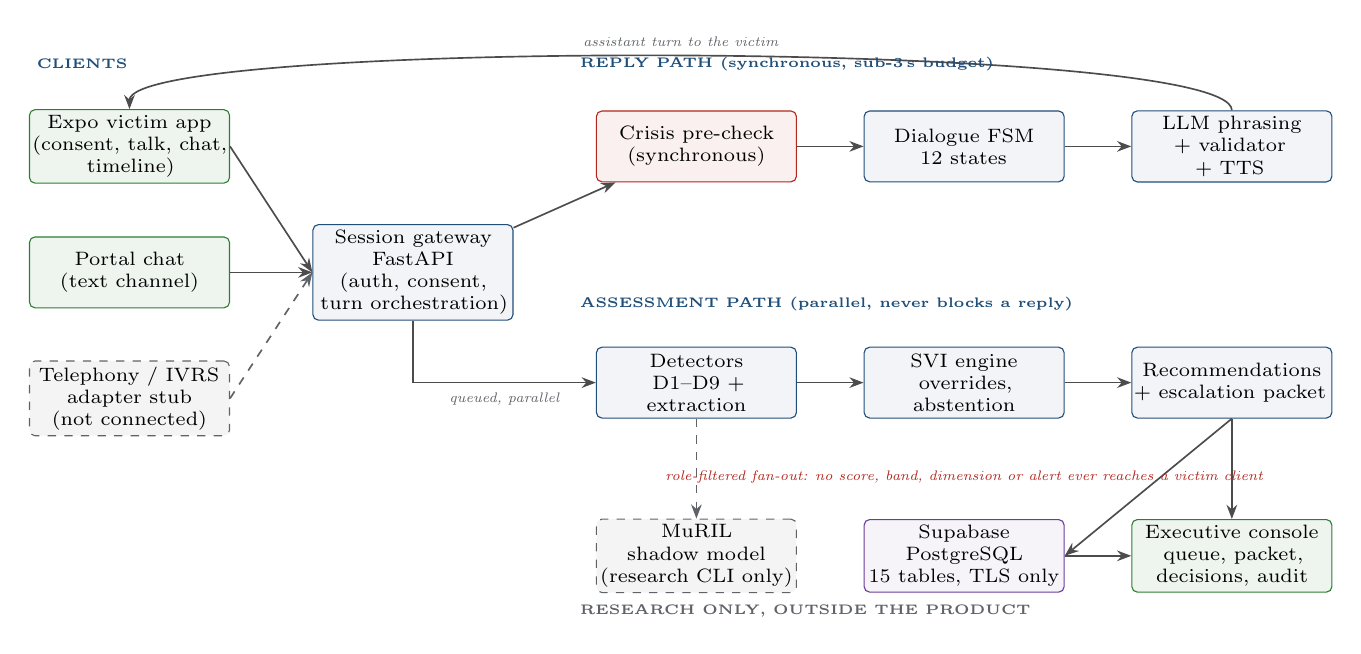
\begin{tikzpicture}[
  font=\scriptsize,
  cli/.style={draw=sahaygreen, rounded corners=2pt, fill=sahaygreen!8, align=center,
              minimum height=9mm, text width=24mm, inner sep=2pt},
  box/.style={draw=sahayblue, rounded corners=2pt, fill=sahayblue!6, align=center,
              minimum height=9mm, text width=24mm, inner sep=2pt},
  crit/.style={box, draw=sahayred, fill=sahayred!7},
  store/.style={draw=sahaypurple, rounded corners=2pt, fill=sahaypurple!6, align=center,
                minimum height=9mm, text width=24mm, inner sep=2pt},
  shd/.style={box, draw=sahaygray, dashed, fill=sahaygray!7},
  arr/.style={-{Stealth[length=1.8mm]}, semithick, draw=black!70},
  darr/.style={arr, dashed, draw=sahaygray},
  lab/.style={font=\tiny\itshape, text=sahaygray, align=center},
  zone/.style={font=\tiny\bfseries, text=sahayblue, align=left, anchor=west},
]
% clients
\node[cli] (app)   at (0,0)      {Expo victim app\\(consent, talk, chat,\\timeline)};
\node[cli] (portal)at (0,-1.6)   {Portal chat\\(text channel)};
\node[shd] (ivrs)  at (0,-3.2)   {Telephony / IVRS\\adapter stub\\(not connected)};
% gateway
\node[box] (gw)    at (3.6,-1.6) {Session gateway\\FastAPI\\(auth, consent,\\turn orchestration)};
% reply path
\node[crit](pre)   at (7.2,0)    {Crisis pre-check\\(synchronous)};
\node[box] (fsm)   at (10.6,0)   {Dialogue FSM\\12 states};
\node[box] (val)   at (14.0,0)   {LLM phrasing\\+ validator\\+ TTS};
% assessment path
\node[box] (det)   at (7.2,-3.0) {Detectors\\D1--D9 + extraction};
\node[box] (svi)   at (10.6,-3.0){SVI engine\\overrides, abstention};
\node[box] (pkt)   at (14.0,-3.0){Recommendations\\+ escalation packet};
% storage and console
\node[store](db)   at (10.6,-5.2){Supabase PostgreSQL\\15 tables, TLS only};
\node[cli] (con)   at (14.0,-5.2){Executive console\\queue, packet,\\decisions, audit};
\node[shd] (shadow)at (7.2,-5.2) {MuRIL shadow model\\(research CLI only)};

\draw[arr] (app.east)    -- (gw.west);
\draw[arr] (portal.east) -- (gw.west);
\draw[darr] (ivrs.east)  -- (gw.west);
\draw[arr] (gw) -- (pre);
\draw[arr] (pre) -- (fsm);
\draw[arr] (fsm) -- (val);
\draw[arr] (val.north) .. controls +(0,0.9) and +(0,0.9) .. node[lab,above]{assistant turn to the victim} (app.north);
\draw[arr] (gw.south) |- node[lab,below,pos=0.75]{queued, parallel} (det.west);
\draw[arr] (det) -- (svi);
\draw[arr] (svi) -- (pkt);
\draw[arr] (pkt) -- (con);
\draw[arr] (pkt.south) -- (db.east);
\draw[arr] (db) -- (con);
\draw[darr] (det.south) -- (shadow.north);
\node[lab, text=sahayred] at (10.6,-4.2) {role-filtered fan-out: no score, band, dimension or alert ever reaches a victim client};
\node[zone] at (-1.3,1.05) {CLIENTS};
\node[zone] at (5.6,1.05)  {REPLY PATH (synchronous, sub-3\,s budget)};
\node[zone] at (5.6,-2.0)  {ASSESSMENT PATH (parallel, never blocks a reply)};
\node[zone, text=sahaygray] at (5.6,-5.9) {RESEARCH ONLY, OUTSIDE THE PRODUCT};
\end{tikzpicture}
\caption{SAHAY-AI system architecture. Solid arrows are live paths; dashed arrows are not connected
in the MVP (telephony) or are research-only (the trained shadow model).}
\label{fig:arch}
\end{figure}

\subsection{Runtime and deployment}
Everything in Table~\ref{tab:runtime} runs on one machine and, apart from the managed database,
entirely offline. The choices were made so that a later move to departmental infrastructure is a
configuration change rather than a rewrite: persistence, the assessment runner, retrieval, speech and
the language model all sit behind adapters with mocks.

\begin{table}[!htbp]
\centering\small
\caption{Runtime profile of the MVP, as configured in the repository.}
\label{tab:runtime}
\begin{tabularx}{\linewidth}{@{}>{\raggedright\arraybackslash}p{3.6cm}X@{}}
\toprule
Layer & Choice and rationale \\
\midrule
API & FastAPI in one process, Pydantic v2 contracts, bound to the LAN so a physical phone can reach it \\
Database & Supabase PostgreSQL over TLS through SQLAlchemy and Alembic. The configuration layer
refuses a non-TLS URL, refuses the pooler port, and refuses SQLite outside an explicit test
environment \\
Background work & In-process assessment runner; assessment cycles run in a worker thread and are
drained on shutdown. Redis and RQ remain deferred \\
Console & React 18, TypeScript, Vite, with a typed mirror of the backend enumerations that a test
compares against the contract \\
Victim app & Expo / React Native (SDK 54) with an offline queue, i18n for Hindi and English, and a
strict event allowlist \\
Speech and text models & Self-hosted and pinned: Whisper Small converted to CTranslate2, Silero VAD,
MuRIL as the text encoder, XLM-R for comparison only. All loaded offline, none on the reply path \\
LLM & Mock adapter by default. The complete dialogue runs with the model disabled \\
Secrets & Environment only; never committed. Tokens and JWT shapes are redacted from logs \\
\bottomrule
\end{tabularx}
\end{table}

\subsection{Data model}
The schema is deliberately boring, because an auditable record is worth more than a clever one.
Fifteen tables carry the case: \code{users}, \code{sessions}, \code{consents}, \code{turns},
\code{cases}, \code{assessments}, \code{alerts}, \code{recommendations}, \code{decisions\_ai},
\code{decisions\_human}, \code{overrides}, \code{timeline\_events}, \code{audit\_log},
\code{policy\_chunks} and \code{latency\_metrics}. Four design rules matter:

\begin{itemize}
  \item \code{decisions\_ai} and \code{decisions\_human} are separate tables, so the record can never
        read as though a machine decided.
  \item \code{overrides} is the authoritative store of band overrides and its \code{reason} column is
        \code{NOT NULL}, enforced again at the endpoint.
  \item \code{timeline\_events} is the authoritative victim-safe timeline, unique per case and dedupe
        key, and carries no assessment field.
  \item \code{audit\_log} is append-only and is an accountability record, not the timeline.
\end{itemize}

\subsection{The contract surface}
Interfaces are frozen in a single document that every team builds against, and a test parses that
document and fails if any copy of the enumerations drifts. The victim event allowlist is the
safety-critical part:
\begingroup\raggedright
\begin{itemize}[itemsep=1pt]
  \item \textbf{A victim client may receive only} \filepath{assistant.turn},
        \filepath{transcript.line}, \filepath{session.status}, \filepath{timeline.update} and
        \filepath{officer.message}.
  \item \textbf{Executive-only, filtered server-side:} \filepath{dimension.update},
        \filepath{alert.safety}, \filepath{case.structured},
        \filepath{action.recommended}, \filepath{safesignal.flag} and
        \filepath{escalation.packet}.
\end{itemize}
\endgroup
%======================================================================
\section{Flows}
\label{sec:flows}

\subsection{The intake conversation}
The dialogue is a 12-state machine (Figure~\ref{fig:fsm}). States are skippable and reorderable: if
the free narrative already answered ``who and when'', that state is skipped, because asking a
distressed person what they just said is the fastest way to lose their trust. The target is 8--12
turns. The chat channel uses the identical machine; text turns simply skip ASR and TTS.

\begin{figure}[!htbp]
\centering
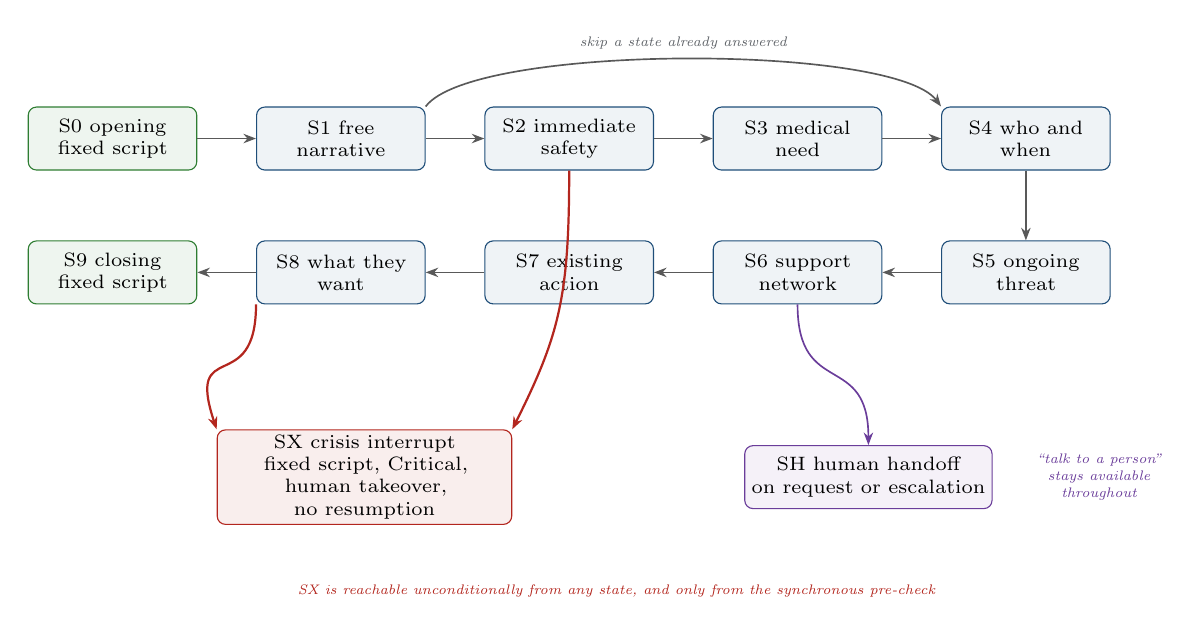
\begin{tikzpicture}[
  font=\scriptsize,
  st/.style={draw=sahayblue, rounded corners=3pt, fill=sahayblue!7, align=center,
             minimum height=8mm, text width=20mm, inner sep=2pt},
  fix/.style={st, draw=sahaygreen, fill=sahaygreen!8},
  crit/.style={st, draw=sahayred, fill=sahayred!8},
  hum/.style={st, draw=sahaypurple, fill=sahaypurple!7},
  arr/.style={-{Stealth[length=1.6mm]}, semithick, draw=black!65},
  crisisarr/.style={arr, draw=sahayred, thick},
  lab/.style={font=\tiny\itshape, text=sahaygray, align=center},
]
\node[fix] (s0) at (0,0)      {S0 opening\\fixed script};
\node[st]  (s1) at (2.9,0)    {S1 free\\narrative};
\node[st]  (s2) at (5.8,0)    {S2 immediate\\safety};
\node[st]  (s3) at (8.7,0)    {S3 medical\\need};
\node[st]  (s4) at (11.6,0)   {S4 who and\\when};
\node[st]  (s5) at (11.6,-1.7){S5 ongoing\\threat};
\node[st]  (s6) at (8.7,-1.7) {S6 support\\network};
\node[st]  (s7) at (5.8,-1.7) {S7 existing\\action};
\node[st]  (s8) at (2.9,-1.7) {S8 what they\\want};
\node[fix] (s9) at (0,-1.7)   {S9 closing\\fixed script};
\node[crit, text width=36mm](sx) at (3.2,-4.3)
  {SX crisis interrupt\\fixed script, Critical,\\human takeover, no resumption};
\node[hum, text width=30mm] (sh) at (9.6,-4.3) {SH human handoff\\on request or escalation};
\draw[arr] (s0) -- (s1); \draw[arr] (s1) -- (s2); \draw[arr] (s2) -- (s3);
\draw[arr] (s3) -- (s4); \draw[arr] (s4) -- (s5); \draw[arr] (s5) -- (s6);
\draw[arr] (s6) -- (s7); \draw[arr] (s7) -- (s8); \draw[arr] (s8) -- (s9);
\draw[arr] (s1.north east) .. controls +(0.6,0.8) and +(-0.6,0.8) ..
  node[lab,above,pos=0.5]{skip a state already answered} (s4.north west);
\draw[crisisarr] (s2.south) .. controls +(0,-1.6) and +(0.6,1.2) .. (sx.north east);
\draw[crisisarr] (s8.south west) .. controls +(0,-1.2) and +(-0.4,1.2) .. (sx.north west);
\node[lab, text=sahayred] at (6.4,-5.75)
  {SX is reachable unconditionally from any state, and only from the synchronous pre-check};
\draw[arr, draw=sahaypurple] (s6.south) .. controls +(0,-1.2) and +(0,1.2) .. (sh.north);
\node[lab, text=sahaypurple, anchor=west] at (11.6,-4.3) {``talk to a person''\\stays available\\throughout};
\end{tikzpicture}
\caption{The dialogue state machine. Green states are fixed pre-approved scripts that are never model
generated; the red state can interrupt from anywhere and never returns to intake.}
\label{fig:fsm}
\end{figure}

\subsection{One turn, end to end}
\label{sec:turnflow}
Figure~\ref{fig:turn} is the order of operations in \filepath{backend/app/services/turn_loop.py}.
That order is a safety invariant, not an implementation detail: the crisis pre-check runs before
dialogue policy, and the validator runs before anything is spoken.

\begin{figure}[!htbp]
\centering
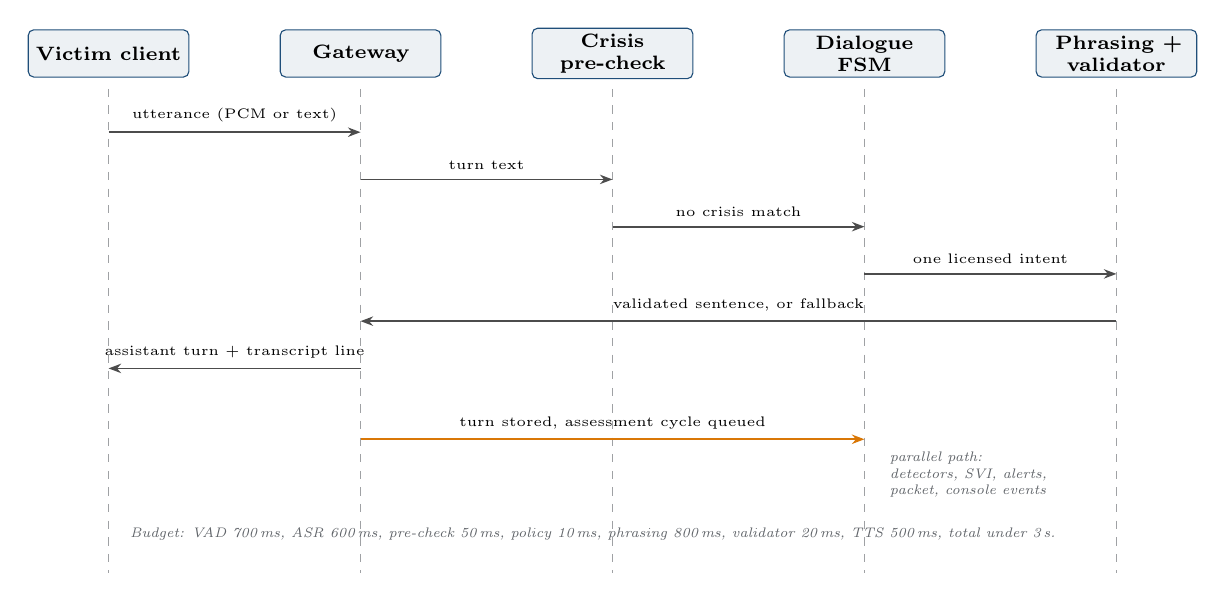
\begin{tikzpicture}[
  font=\scriptsize,
  lifeline/.style={draw=sahaygray!60, dashed},
  head/.style={draw=sahayblue, fill=sahayblue!8, rounded corners=2pt, align=center,
               text width=19mm, minimum height=6mm, inner sep=2pt, font=\scriptsize\bfseries},
  msg/.style={-{Stealth[length=1.6mm]}, semithick, draw=black!70, font=\tiny},
  note/.style={font=\tiny\itshape, text=sahaygray, align=left},
]
\def\lx{0} \def\gx{3.2} \def\px{6.4} \def\dx{9.6} \def\vx{12.8}
\node[head] (L) at (\lx,0) {Victim client};
\node[head] (G) at (\gx,0) {Gateway};
\node[head] (P) at (\px,0) {Crisis\\pre-check};
\node[head] (D) at (\dx,0) {Dialogue\\FSM};
\node[head] (V) at (\vx,0) {Phrasing +\\validator};
\foreach \x in {\lx,\gx,\px,\dx,\vx} { \draw[lifeline] (\x,-0.45) -- (\x,-6.6); }
\draw[msg] (\lx,-1.0) -- node[above]{utterance (PCM or text)} (\gx,-1.0);
\draw[msg] (\gx,-1.6) -- node[above]{turn text} (\px,-1.6);
\draw[msg] (\px,-2.2) -- node[above]{no crisis match} (\dx,-2.2);
\draw[msg] (\dx,-2.8) -- node[above]{one licensed intent} (\vx,-2.8);
\draw[msg] (\vx,-3.4) -- node[above]{validated sentence, or fallback} (\gx,-3.4);
\draw[msg] (\gx,-4.0) -- node[above]{assistant turn + transcript line} (\lx,-4.0);
\draw[msg, draw=sahayorange] (\gx,-4.9) -- node[above]{turn stored, assessment cycle queued} (\dx,-4.9);
\node[note, anchor=west] at (\dx+0.2,-5.35) {parallel path:\\detectors, SVI, alerts,\\packet, console events};
\node[note, anchor=west] at (\lx+0.15,-6.1) {Budget: VAD 700\,ms, ASR 600\,ms, pre-check 50\,ms, policy 10\,ms, phrasing 800\,ms, validator 20\,ms, TTS 500\,ms, total under 3\,s.};
\end{tikzpicture}
\caption{One intake turn. The assessment cycle is queued after the reply has already been sent, so a
slow model can never delay the assistant.}
\label{fig:turn}
\end{figure}

\subsection{The crisis interrupt}
\label{sec:crisisflow}
This is the flow the project is judged on. It is unconditional, it is not a model decision, and it
does not resume.

\begin{enumerate}[itemsep=1pt]
  \item Every utterance, in every state, goes through the synchronous pre-check before dialogue
        policy. It uses high-recall Hindi, English and romanised Hinglish lexicons with clause-scoped
        negation and quotation handling, because a false alarm costs an officer thirty seconds and a
        miss costs far more.
  \item On a match the session moves to state SX in code. The band is forced to Critical, a crisis
        alert is raised with \code{requires\_ack}, the case jumps to the top of the queue with an
        audible cue, and a takeover is requested.
  \item The assistant speaks only the fixed, pre-approved SX script: it acknowledges, says plainly
        that a person will speak with them now, and asks them to stay. No advice, no questions, no
        assessment.
  \item Intake does not resume. Only a human takeover continues the session.
  \item \textbf{Fail-closed today:} the SX, S0, S9 and SH scripts are not yet written and reviewed,
        so the assistant says \emph{nothing} in those states and the event is audited as
        \code{fixed\_script.unavailable}. Nothing unreviewed is ever spoken to a victim. Writing and
        review by a counsellor is the outstanding item, tracked in the repository.
\end{enumerate}

\subsection{The assessment cycle}
\label{sec:assessflow}
A cycle is keyed by the case and the number of victim turns heard, so running it twice writes nothing
the second time. It reads the turns, runs the pure deterministic pipeline in a worker thread,
persists exactly one assessment row per cycle, updates the case band with its cause, upserts alerts
(unique per case and type) and recommendations (unique per case and pathway), and publishes
executive-only events. It never speaks to the victim and never triggers the crisis interrupt.

Human authority is enforced here too: once an officer overrides the band, later cycles keep assessing
but do not replace the officer's band --- except that a hard safety override still escalates to
Critical, which always wins.

\subsection{Scoring, overrides and abstention}
\label{sec:svi}
The index is a weighted sum over nine dimensions (Table~\ref{tab:svi}), each score on 0--100 and each
carrying the turn ids that justify it:
\[
\mathrm{SVI} \;=\; \frac{\sum_{i \in \text{available}} w_i\, s_i}{\sum_{i \in \text{available}} w_i},
\qquad
\text{bands: } 0\text{--}29\ \text{Low},\; 30\text{--}54\ \text{Moderate},\; 55\text{--}74\ \text{High},\; 75\text{--}100\ \text{Critical}.
\]

\begin{table}[!htbp]
\centering\small
\caption{The nine dimensions and their provisional weights, pending an expert calibration study.}
\label{tab:svi}
\begin{tabular}{@{}llc@{\hspace{0.6cm}}llc@{}}
\toprule
Dim & Meaning & Weight & Dim & Meaning & Weight \\
\midrule
D1 & Immediate safety threat & 0.22 & D6 & Isolation, boycott, displacement & 0.08 \\
D2 & Crisis / self-harm language & 0.18 & D7 & Medical urgency & 0.08 \\
D3 & Fear, intimidation, threats & 0.13 & D8 & Legal urgency & 0.06 \\
D4 & Acute distress (acoustic) & 0.12 & D9 & Communication safety & 0.05 \\
D5 & Trauma-associated indicators & 0.08 & & & \\
\bottomrule
\end{tabular}
\end{table}

Three behaviours distinguish this from a naive score:
\begin{itemize}
  \item \textbf{Hard overrides beat weights.} A confirmed immediate danger or crisis forces Critical
        regardless of the sum, and the assessment records which override applied.
  \item \textbf{Structural renormalisation, never zero-filling.} On a typed channel the acoustic
        dimension has no measurement path at all, so the denominator becomes 0.88 and the console
        states that D4 was unavailable. D4 is never reported as measured and never set to zero. Poor
        audio or a runtime failure does \emph{not} renormalise: it abstains.
  \item \textbf{Abstention is a first-class output.} Aggregate confidence below 0.45, poor audio or
        low language confidence returns \emph{Needs Human Assessment} with no score anywhere, not in
        the packet, the queue or the trajectory. Consent declined suppresses scoring entirely.
\end{itemize}

\subsection{Escalation and the human decision}
\label{sec:escalationflow}
Figure~\ref{fig:case} is the case lifecycle. Every transition is a human action except the first.

\begin{figure}[!htbp]
\centering
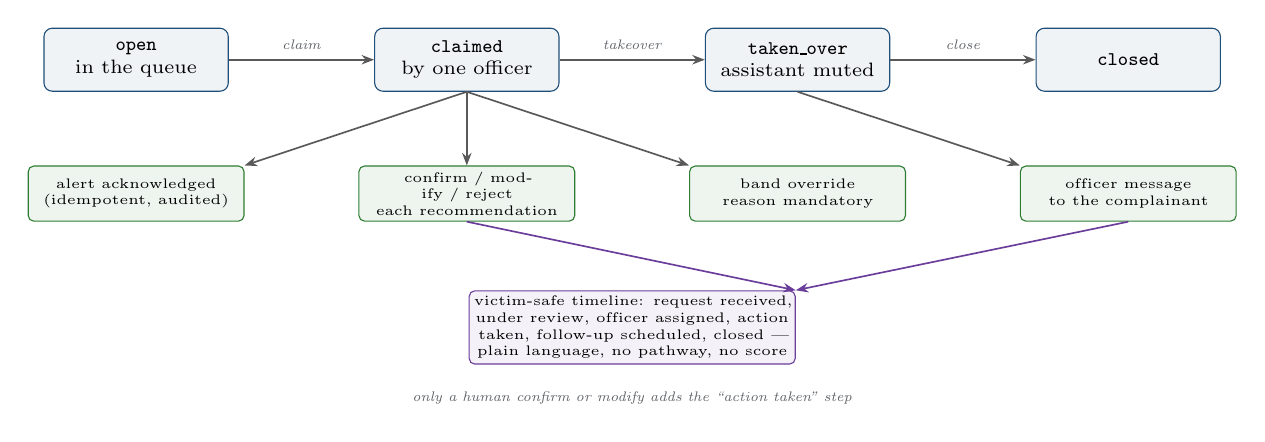
\begin{tikzpicture}[
  font=\scriptsize,
  st/.style={draw=sahayblue, rounded corners=3pt, fill=sahayblue!7, align=center,
             minimum height=8mm, text width=22mm, inner sep=2pt},
  act/.style={draw=sahaygreen, rounded corners=2pt, fill=sahaygreen!8, align=center,
              minimum height=7mm, text width=26mm, inner sep=2pt, font=\tiny},
  arr/.style={-{Stealth[length=1.6mm]}, semithick, draw=black!65},
  lab/.style={font=\tiny\itshape, text=sahaygray, align=center},
]
\node[st] (open)  at (0,0)    {\code{open}\\in the queue};
\node[st] (clm)   at (4.2,0)  {\code{claimed}\\by one officer};
\node[st] (tko)   at (8.4,0)  {\code{taken\_over}\\assistant muted};
\node[st] (cls)   at (12.6,0) {\code{closed}};
\draw[arr] (open) -- node[lab,above]{claim} (clm);
\draw[arr] (clm) -- node[lab,above]{takeover} (tko);
\draw[arr] (tko) -- node[lab,above]{close} (cls);
\node[act] (a1) at (0,-1.7)   {alert acknowledged\\(idempotent, audited)};
\node[act] (a2) at (4.2,-1.7) {confirm / modify / reject\\each recommendation};
\node[act] (a3) at (8.4,-1.7) {band override\\reason mandatory};
\node[act] (a4) at (12.6,-1.7){officer message\\to the complainant};
\draw[arr] (clm.south) -- (a1.north east);
\draw[arr] (clm.south) -- (a2.north);
\draw[arr] (clm.south) -- (a3.north west);
\draw[arr] (tko.south) -- (a4.north west);
\node[act, text width=40mm, draw=sahaypurple, fill=sahaypurple!7] (tl) at (6.3,-3.4)
  {victim-safe timeline: request received, under review, officer assigned, action taken,
   follow-up scheduled, closed --- plain language, no pathway, no score};
\draw[arr, draw=sahaypurple] (a2.south) -- (tl.north east);
\draw[arr, draw=sahaypurple] (a4.south) -- (tl.north east);
\node[lab] at (6.3,-4.3) {only a human confirm or modify adds the ``action taken'' step};
\end{tikzpicture}
\caption{Case lifecycle and the officer actions attached to each state. Every write is
executive-only; a supervisor token is read-only and gets 403.}
\label{fig:case}
\end{figure}

The packet the officer opens has ten sections: header, assessment summary with the dimension
breakdown and confidence, safety alerts requiring acknowledgement, the structured case record with
every field linked to its source utterance, the full two-sided transcript, the evidence panel, the
SVI trajectory, recommended pathways with rationale and policy citation, an uncertainty block with
equal prominence to the score, and the decision area. The target is a decision in under 90 seconds
without listening to a recording.

\subsection{What the complainant sees}
\label{sec:timeline}
The victim surface is deliberately thin: language choice, consent with AI disclosure, talk or chat,
and a status timeline. The timeline contains no assessment field, and an automated test asserts the
response contains none of \code{svi}, \code{band}, \code{dimension}, \code{alert} or
\code{confidence}. Labels are process facts in plain language --- ``an officer has taken action on
your request'' --- never ``counselling pathway initiated'', and never the band.

\subsection{Degraded and edge flows}
A triage system is judged on what it does when something breaks, so the degraded paths are
implemented and tested rather than documented as future work (Table~\ref{tab:degraded}).

\begin{table}[!htbp]
\centering\small
\caption{Behaviour when something goes wrong. Each row is implemented and covered by tests.}
\label{tab:degraded}
\begin{tabularx}{\linewidth}{@{}>{\raggedright\arraybackslash}p{3.8cm}X@{}}
\toprule
Situation & Behaviour \\
\midrule
Consent declined & The text is kept for a person to read; no AI analysis runs at all: no score, no
alerts from the pipeline, no recommendations \\
Model or LLM unavailable & The intake completes from pre-written per-intent fallbacks in both
languages; the LLM-off walk is part of the evaluation and passes \\
Fixed script not yet approved & The assistant stays silent in that state and the event is audited;
nothing unreviewed is spoken \\
Poor or unreadable input & Abstention: \emph{Needs Human Assessment}, no score published anywhere \\
Network loss on the phone & The victim app queues turns and resumes from the last acknowledged
sequence number; the server de-duplicates \\
Repeated processing of a turn & Idempotency keys on turns, assessments, alerts, recommendations,
timeline events and acknowledgements mean a replay writes nothing new \\
Shadow model fires, errors, hangs or returns rubbish & The deterministic output is unchanged: proved
across 60 records under seven fault conditions with zero mismatches \\
\bottomrule
\end{tabularx}
\end{table}

%======================================================================
\section{Technical approach and why}
\label{sec:approach}

\subsection{Why a deterministic machine phrases through a model, not the reverse}
\label{sec:guardrails}
A free-form assistant talking to trauma victims fails in ways that are obvious in hindsight: it gives
legal advice, promises an arrest, asks for forensic detail, or comforts with ``don't worry''. Our
design makes those outcomes structurally impossible rather than statistically unlikely. The state
machine picks the intent; the model may only rephrase it; a validator with ten checks (length,
unlicensed question, advice, promise, diagnosis, banned comfort, detail-seeking, blame, language,
disclosure) runs before synthesis, and a rejection falls back to pre-written text. The rejection rate
itself is a tracked metric.

\subsection{Why a transparent weighted index, not a learned score}
\label{sec:whyindex}
An officer must be able to see why a case is Critical, and a supervisor must be able to audit it. A
weighted sum over nine evidence-linked dimensions gives that for free, is calibratable by experts
later, and abstains cleanly. A learned regressor trained on fictional data would be unexplainable,
uncalibrated, and impossible to defend without outcome data from real triage. Our own experiment
supports this choice: the trained model we did build underperformed the deterministic pipeline on the
exposed fixtures (Section~\ref{sec:shadow}).

\subsection{Why MuRIL for text}
\label{sec:whymuril}
Helpline text is code-mixed and frequently romanised. MuRIL is pre-trained on Indian-language text
with transliterated pairs and reports a large advantage exactly there: 48.9 against mBERT's 21.1 on
transliterated test sets, and 68.6 against 59.1 on native-script sets~\cite{khanuja2021}. Our own
measurement agrees on efficiency: the pinned MuRIL tokeniser needs 0.246 tokens per character on
Hindi against XLM-R's 0.319, and 0.259 against 0.294 on Hinglish, with a zero unknown-token rate.
That is roughly 23\% fewer tokens per Hindi character, which is 23\% more context inside the same
128-token window.

\subsection{Why VAD gates the speech model}
\label{sec:whyvad}
During qualification, Whisper Small produced fluent Hindi text from five seconds of \emph{silence}
(median 186 characters) and from a pure tone (148 characters) when forced to decode. On a helpline,
hallucinated text is not a quality problem, it is a safety problem. So Silero VAD is an enforced
precondition in code: the transcribe method has no default for its speech intervals, validates every
interval before decoding, decodes only the audio inside accepted intervals, and skips the model
entirely when no speech is found. An unguarded path exists only inside the benchmark module and is
statically fenced by a test.

\subsection{Why the acoustic dimension is a within-caller rule}
\label{sec:d4}
The PS asks for pitch variation and emotional indicators, and the literature supports that acoustic
features carry trauma-relevant signal~\cite{hu2024,islam2024}. It also argues for caution: the best
available speech-based PTSD study explains about a tenth of the variance in symptom severity
($R^2 = 0.10$) even with clinical recordings~\cite{hu2024}. So D4 is a transparent rule rather than a
learned score: it compares a caller's later turns with that caller's own first turns, counts only
upward change, needs three usable voice turns, caps its confidence at 0.6, and abstains on poor audio.
On a typed channel D4 remains structurally unavailable and the index renormalises. A speech-emotion
model may later supply at most 30\% of D4, only after passing a gate on the team's own recordings
(Section~\ref{sec:ser}).

\subsection{The source-label firewall}
\label{sec:firewall}
Public corpora label other things: subreddit of origin, stress, sentiment, hate speech, emotion. None
of these is a SAHAY safety label, and the repository refuses every automatic mapping from one to the
other --- stress is not crisis, a non-suicide subreddit label is not ``safe'', hate speech is not
continuing threat, emotion is not acoustic distress, and no source label may ever become an SVI, a
band or a routing decision. Under decision EXT-129 a source label may act as a \emph{weak training
label} through a separate training-only path, tagged \code{weak\_supervision\_from\_source\_label}
with its caveat, and never for diagnosis, the SVI, the band, routing or D4. This is why the project
can train on public data (Section~\ref{sec:stagew}) without laundering it into safety ground truth.

\subsection{Privacy, security and DPDP posture}
\label{sec:privacy}
Consent precedes capture, and declining it suppresses scoring entirely. All speech and NLP run
locally, so no victim audio leaves the deployment. The database layer refuses a non-TLS connection.
Access is JWT with role-based authorisation, and a victim session token is scoped to its own session
and rejected by every console route. Logs redact tokens and JWT shapes, validation errors never echo
the submitted text, and a 500 never returns a stack trace or case text. Against the Digital Personal
Data Protection Act 2023 and its 2025 Rules~\cite{meity2023}, the design already implements notice
and consent, purpose limitation (the victim client cannot receive assessment data), local processing,
and retention separation between audio and derived case data; breach processes, a consent-manager
integration and a formal lawful-basis assessment are production work, listed in
Section~\ref{sec:roadmap}.

%======================================================================
% AI models: what we built, trained and measured (included from local-research-analysis.tex).
% Every number here comes from a committed result file or a private run report; sources are
% listed in the evidence index. Evidence classes are stated beside each result.
%======================================================================
\section{AI models: what we built, trained and measured}
\label{sec:models}

This section is the core of the technical work. It covers every model and model-like component in
the system: what it is, how it was trained, what it measured, and whether it is allowed to affect a
victim. One rule runs through all of it. The deterministic pipeline (crisis pre-check, rule-based
detectors, output validator and SVI engine) is \textbf{authoritative}. Every trained model is
measured against it and runs in \textbf{shadow} until it beats that pipeline on independent
evidence --- which does not yet exist, because the locked evaluation set is still empty.

\subsection{Model inventory and roles}

\begin{table}[!htbp]
\centering\footnotesize
\caption{Every AI component, its role and its current status.}
\label{tab:modelinv}
\begin{tabularx}{\linewidth}{@{}>{\raggedright\arraybackslash}p{3.2cm}>{\raggedright\arraybackslash}p{5.6cm}X@{}}
\toprule
Component & What it is & Status \\
\midrule
Crisis pre-check and detectors & Phrase lexicons with clause-scoped negation, attribution cues and an
explicit spelling map; English, Hindi, Hinglish & \textbf{Authoritative} \\
Output validator & 87 phrase rules and licensed-question checks before any sentence is spoken &
\textbf{Authoritative} \\
SVI engine & Weighted sum, hard overrides, abstention & \textbf{Authoritative}; weights provisional \\
Speech-to-text & Whisper Small (CTranslate2) behind Silero VAD, in a loopback-only service & In the
voice path \\
D4 voice distress & Rule over pitch, loudness and pauses relative to the caller's own first turns &
Wired; unvalidated \\
Speech emotion (SER) & emotion2vec+ large, Whisper-encoder head, WavLM Base+; prosody baseline &
Shadow; excluded from D4 until its gate \\
Text affect & MuRIL (domain-adapted), fine-tuned for five affect classes & Shadow \\
Shadow safety detector & MuRIL with nine heads, fictional supervision plus weak source labels &
Shadow; \code{rejected\_for\_product\_integration} \\
Interpretable baseline & Standard-library logistic regression on hashed n-grams & Comparison only \\
Voice output & Human-recorded fixed scripts; built-in offline Windows voice for validated turns &
Wired; silent until scripts are approved \\
\bottomrule
\end{tabularx}
\end{table}

All training ran on the demo laptop (Ryzen 7 7840HS, RTX 4060 8~GB, 32~GB RAM), offline, with
network access blocked in code. Weights stay in a private root outside Git and are never loaded by
the backend, console or victim app.

\subsection{Speech recognition service}
Speech recognition runs as a separate local process bound to \code{127.0.0.1} and reached through a
backend adapter (contract PC-11: \code{POST /sessions/\{id\}/audio}). The pipeline decodes the
upload, finds speech regions with Silero VAD, runs Whisper Small on those regions only, and returns
the transcript with a confidence summary, audio-quality measures and prosody for D4. Low confidence
or poor audio makes the assessment abstain. A 16~kHz mono PCM WAV now bypasses the general decoder:
the samples are identical and decoding drops from about 50~ms to 0.55~ms per clip.

\begin{table}[!htbp]
\centering\small
\caption{Measured voice-turn latency (70 turns; laptop GPU; synthetic Indian-English speech from
built-in Windows voices). Evidence: synthetic speech, server-side only.}
\label{tab:m2}
\begin{tabular}{@{}lccc@{}}
\toprule
Stage & p50 & p95 & Budget \\
\midrule
Speech-to-text request & 463\,ms & 572\,ms & 600\,ms \\
Reply path after the transcript (pre-check, policy, reply) & 9\,ms & 13\,ms & --- \\
Whole server-side voice turn & 476\,ms & 581\,ms & --- \\
Offline English voice, whole reply & 31\,ms & 38\,ms & 500\,ms \\
\midrule
Server p95 plus the configured 700\,ms end-of-speech wait & \multicolumn{2}{c}{1.28\,s} & 3\,s \\
\bottomrule
\end{tabular}
\end{table}

Word error rate on real Hindi and English speech (M6) is not yet measured: it needs Common Voice
Hindi or team recordings. The 0.0 WER on the synthetic benchmark speech is a sanity check, not M6.

\subsection{Speech emotion recognition}
\label{sec:ser}
The problem statement asks for emotional indicators in voice. We trained and compared four candidate
families on the two acted English corpora available to us, RAVDESS (864 usable clips, 24 actors) and
CREMA-D (6{,}097 usable clips, 91 actors), with actor-disjoint, sex-stratified splits and five affect
classes (neutral, happy, sad, angry, fearful). The metric is unweighted average recall (UAR, chance
0.20) with bootstrap 95\% intervals.

\begin{table}[!htbp]
\centering\footnotesize
\caption{Speech-emotion candidates on unseen actors. ``Possibly seen'': emotion2vec+'s pre-training
is believed to include these corpora, so its lead may be memory rather than skill.}
\label{tab:ser}
\setlength{\tabcolsep}{5pt}
\begin{tabular}{@{}lllll@{}}
\toprule
Candidate & Evidence & CREMA-D test (873) & RAVDESS test (141) & Cross-corpus \\
\midrule
emotion2vec+ head & possibly seen & 0.784 [0.756, 0.809] & 0.796 [0.721, 0.863] & 0.872 \\
emotion2vec+ zero-shot & possibly seen & 0.766 & 0.809 & 0.868 \\
Whisper-encoder head & clean & 0.767 [0.741, 0.794] & 0.784 [0.710, 0.854] & 0.706 \\
WavLM Base+ fine-tune & clean & 0.758 [0.732, 0.783] & 0.758 [0.681, 0.832] & 0.447 \\
Prosody logistic, speaker-normalised & clean & 0.580 [0.549, 0.611] & 0.432 [0.359, 0.509] & 0.487 \\
Prosody logistic, pooled & clean & 0.527 & 0.357 & 0.345 \\
\bottomrule
\end{tabular}
\end{table}

\begin{figure}[!htbp]
\centering
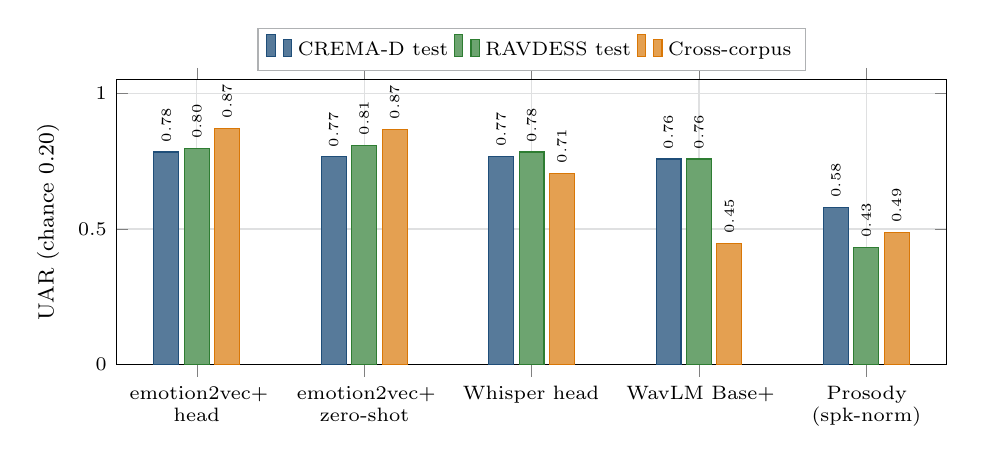
\begin{tikzpicture}
\begin{axis}[sahay, ybar, bar width=9pt, width=\linewidth, height=5.2cm,
  ymin=0, ymax=1.05, ylabel={UAR (chance 0.20)},
  symbolic x coords={e2vh,e2vz,whis,wavlm,pros},  xtick=data,
  xticklabels={emotion2vec+ head, emotion2vec+ zero-shot, Whisper head, WavLM Base+, Prosody (spk-norm)},
  x tick label style={font=\scriptsize, align=center, text width=2.2cm},
  enlarge x limits=0.12,
  nodes near coords={\pgfmathprintnumber[fixed,fixed zerofill,precision=2]{\pgfplotspointmeta}},
  nodes near coords style={font=\tiny, rotate=90, anchor=west},
  legend style={at={(0.5,1.03)}, anchor=south, legend columns=3}]
\addplot[fill=sahayblue!75, draw=sahayblue] coordinates {(e2vh,0.784) (e2vz,0.766) (whis,0.767) (wavlm,0.758) (pros,0.580)};
\addplot[fill=sahaygreen!70, draw=sahaygreen] coordinates {(e2vh,0.796) (e2vz,0.809) (whis,0.784) (wavlm,0.758) (pros,0.432)};
\addplot[fill=sahayorange!70, draw=sahayorange] coordinates {(e2vh,0.872) (e2vz,0.868) (whis,0.706) (wavlm,0.447) (pros,0.487)};
\legend{CREMA-D test, RAVDESS test, Cross-corpus}
\end{axis}
\end{tikzpicture}
\caption{Speech-emotion UAR. The three neural candidates overlap within their intervals on acted
English; WavLM does not transfer across corpora; speaker normalisation helps the prosody baseline by
0.05--0.14, which is the evidence behind D4's in-session baseline.}
\label{fig:ser}
\end{figure}

\noindent Findings: the neural candidates cannot be separated on acted English; ``fearful'' is the
weakest class for every neural model (recall 0.49--0.62), and it is the class that matters most here;
and nothing is measured on Hindi, telephone audio or real distress. Speech emotion therefore stays out
of the score. It may contribute at most 30\% of D4, and only after a promotion gate on the team's own
Hindi and English recordings (UAR $\ge$ 0.45, no class recall below 0.20, a neutral control).

\subsection{D4: voice distress as a within-caller rule}
D4 is no longer empty. It is a transparent rule: each later voice turn is compared with the same
caller's first two usable turns on median pitch, pitch variability, loudness and pause ratio, in
units of that caller's own spread, and only \emph{upward} change counts --- a flatter or quieter voice
is never read as calm. D4 needs at least three usable voice turns, its confidence is capped at 0.6,
and poor audio excludes a turn and makes the assessment abstain. A SAFE-SIGNAL prompt asks the officer
to verify whenever voice distress and text severity differ by more than 40 points; it never changes
the band. The rule is \textbf{unvalidated}: its weights and scale are design choices, and validating it
needs team recordings and expert review.

\subsection{Text affect with MuRIL}
The text model reads five affect classes from one utterance in Hindi, romanised Hinglish or English,
trained on EmoInHindi (Hindi dialogue) and GoEmotions (English). Our first corpus \textbf{leaked}: 84\%
of its test sentences appeared verbatim in training because EmoInHindi reuses template lines, and it
scored about 0.94. We declared those numbers void and rebuilt the corpus sentence-disjoint, grouping
exact and near duplicates (Jaccard $\ge$ 0.8) into a single split.

\begin{table}[!htbp]
\centering\footnotesize
\caption{Text-affect UAR on the sentence-disjoint test sets, with bootstrap 95\% intervals. Hinglish is
machine-transliterated from the Hindi test set.}
\label{tab:textaffect}
\setlength{\tabcolsep}{3pt}
\begin{tabularx}{\linewidth}{@{}>{\raggedright\arraybackslash}p{3.1cm}*{4}{>{\centering\arraybackslash}X}@{}}
\toprule
Encoder & Hindi (778) & Hinglish (777) & Hindi user turns (495) & English (2{,}000) \\
\midrule
\textbf{MuRIL, domain-adapted} (selected) & 0.745 [0.709, 0.779] & 0.699 [0.661, 0.734] & 0.707 & 0.812 [0.784, 0.839] \\
MuRIL base & 0.742 [0.706, 0.778] & 0.713 [0.674, 0.751] & 0.703 & 0.815 [0.788, 0.845] \\
XLM-R base & 0.748 [0.711, 0.782] & 0.705 [0.668, 0.742] & 0.710 & 0.805 [0.774, 0.835] \\
\bottomrule
\end{tabularx}
\end{table}

\noindent The three encoders overlap on every language, so no encoder is better on this evidence;
MuRIL was kept by the predeclared rule. ``Sad'' is the weakest class in Hindi (recall 0.59, and 0.44
on user turns). The model is shadow-only until its licences are confirmed and it passes a gate on
human-written Hinglish.

\subsection{The shadow safety detector (Stage W)}
\label{sec:stagew}
Stage W asks whether labels borrowed from public data help a MuRIL detector catch what the rules miss.
It has nine logits --- the eight detector categories and a \code{d5\_text\_distress} head --- and a
masked focal loss, so a borrowed row teaches only its own label. Three arms were fixed before
training: \textbf{W0} fictional corpus only; \textbf{W1} adds Reddit crisis posts (subreddit of origin)
and Dreaddit stress; \textbf{W2} also adds a hate-speech label as a proxy for threat. Selection used
fictional validation only.

\begin{table}[!htbp]
\centering\footnotesize
\caption{Stage W on corpus \code{7b-v1} (seed 13 per arm, plus two more seeds for the winner W2).
Weak-test AUROC is against the borrowed labels; exposed micro F1 is on SAHAY's published fixtures.}
\label{tab:stagew}
\setlength{\tabcolsep}{4pt}
\begin{tabularx}{\linewidth}{@{}>{\raggedright\arraybackslash}p{3.3cm}*{4}{>{\centering\arraybackslash}X}@{}}
\toprule
Run & Holdout macro F1 & Crisis recall hi / Hinglish & AUROC crisis / threat / D5 & Exposed F1 dev / cand \\
\midrule
W0 & 0.680 & 0.76 / 0.73 & 0.84 / 0.40 / --- & 0.53 / 0.48 \\
W1 & 0.751 & 0.97 / 0.92 & 0.99 / 0.36 / 0.80 & 0.51 / 0.58 \\
W2, seed 13 (selected) & 0.733 & 0.94 / 0.84 & 0.99 / 0.92 / 0.83 & 0.60 / 0.58 \\
W2, seed 42 & 0.842 & 0.98 / 0.98 & 0.99 / 0.91 / 0.82 & 0.52 / 0.48 \\
W2, seed 97 & 0.788 & 0.86 / 0.75 & 0.99 / 0.91 / 0.82 & 0.50 / 0.55 \\
\midrule
Deterministic rules & --- & --- & recall 0.38 / 0.00 / 0.10 & \textbf{0.93 / 0.88} \\
\bottomrule
\end{tabularx}
\end{table}

\begin{figure}[!htbp]
\centering
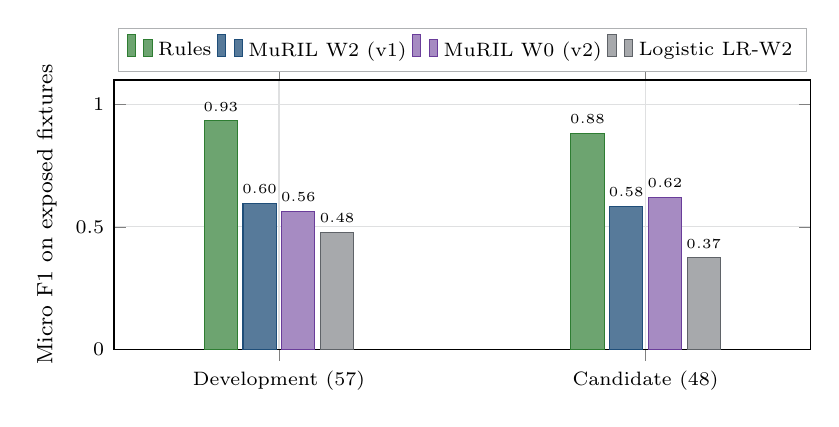
\begin{tikzpicture}
\begin{axis}[sahay, ybar, bar width=12pt, width=0.86\linewidth, height=5.0cm,
  ymin=0, ymax=1.1, ylabel={Micro F1 on exposed fixtures},
  symbolic x coords={dev,cand}, xtick=data, xticklabels={Development (57), Candidate (48)},
  enlarge x limits=0.45,
  nodes near coords={\pgfmathprintnumber[fixed,fixed zerofill,precision=2]{\pgfplotspointmeta}},
  nodes near coords style={font=\tiny},
  legend style={at={(0.5,1.03)}, anchor=south, legend columns=4}]
\addplot[fill=sahaygreen!70, draw=sahaygreen] coordinates {(dev,0.933) (cand,0.881)};
\addplot[fill=sahayblue!75, draw=sahayblue] coordinates {(dev,0.595) (cand,0.584)};
\addplot[fill=sahaypurple!60, draw=sahaypurple] coordinates {(dev,0.563) (cand,0.619)};
\addplot[fill=sahaygray!55, draw=sahaygray] coordinates {(dev,0.477) (cand,0.373)};
\legend{Rules, MuRIL W2 (v1), MuRIL W0 (v2), Logistic LR-W2}
\end{axis}
\end{tikzpicture}
\caption{On SAHAY's own fixtures the deterministic rules lead every trained model. Exposed-regression
evidence; none of these fixtures is independent.}
\label{fig:stagew}
\end{figure}

\noindent What Stage W shows. Borrowed labels clearly help on text like their sources (crisis AUROC
0.84 to 0.99) and even lift Hindi and Hinglish crisis recall on the fictional holdout, although every
borrowed source is English. On SAHAY's fixtures, however, the model stays far below the rules and
raises 18--25 false positives. It catches five candidate fixture-labels the rules miss, including an
indirect method-and-plan statement, but on ten indirect-wording probes it fires on six of seven crisis
probes \emph{and} on all three harmless controls (``I won't be here tomorrow, I'm visiting my
sister''). It is not usable as a crisis signal. It stays a second opinion, and the crisis pre-check
remains the only crisis authority.

\subsection{The interpretable baseline and the corpus shortcut}
A standard-library logistic regression trained on exactly the same data (AE-15) scored 0.48--0.50
holdout macro F1 against MuRIL's 0.73, and 0.24--0.48 exposed micro F1. It also found a flaw: its
strongest crisis and coercion features were fragments of the \code{[SEP]} marker that joins turns. In
corpus \code{7b-v1}, every multi-turn record carried at least one risk label (911 of 911 in train),
so ``has several turns'' predicted ``risky''. We built \code{7b-v2}, which keeps every v1 record and
adds one-positive and all-negative multi-turn records, retrained every arm (R10), and cross-evaluated
both generations of checkpoints on the new holdout.

\begin{table}[!htbp]
\centering\footnotesize
\caption{The shortcut check: v1 and v2 checkpoints on the \code{7b-v2} holdout, by record kind.
Evidence: synthetic development.}
\label{tab:shortcut}
\setlength{\tabcolsep}{4pt}
\begin{tabularx}{\linewidth}{@{}>{\raggedright\arraybackslash}p{3.3cm}*{4}{>{\centering\arraybackslash}X}@{}}
\toprule
Checkpoint & Single-turn F1 & One risky + one harmless turn F1 & False alarms, harmless single & False alarms, harmless multi \\
\midrule
v1 W0 & 0.638 & 0.343 & 2.3\% & 2.4\% \\
v1 W2 (v1 selected) & 0.696 & 0.422 & 3.8\% & 2.4\% \\
v2 W0 (v2 selected) & 0.696 & 0.691 & 7.8\% & 17.4\% \\
v2 W2 & 0.743 & 0.790 & 3.8\% & 7.8\% \\
\bottomrule
\end{tabularx}
\end{table}

\noindent The result corrected our own expectation. MuRIL did \emph{not} learn the crude shortcut ---
v1 models fire on only 2.4\% of harmless multi-turn records; only the linear model did. The real v1
weakness was mixed multi-turn conversations (0.34--0.42 macro F1), which v2 training fixes (0.69--0.79)
at the cost of more false alarms. On SAHAY's fixtures nothing changed materially (v2 W0: 0.56 / 0.62).
Per-label rates are only partly balanced in \code{7b-v2} (coercion 0.25 against 0.15), which a future
version can correct.

\subsection{Upgrades to the authoritative rules}
The rule-based detectors improved during this phase, each change a reviewed-pending draft:
\begin{itemize}
  \item \textbf{Anxiety and low mood (D5).} First-person anxiety and low-mood phrasing in three
        languages, as linguistic indicators, never a diagnosis, with hopelessness wording deliberately
        left to the crisis lexicon.
  \item \textbf{Misspelt imminent return.} An explicit spelling map (``wil'', ``tonite'', ``wapis'')
        and ``come back tonight'' as imminent danger. Dev critical misses went from 1 of 17 to
        \textbf{0 of 17}.
  \item \textbf{Conditional coercion.} ``Agar complaint wapas nahi li to\ldots'' is a threat, not a
        denial. Candidate coercion recall went from 0.40 to \textbf{0.60}.
\end{itemize}
No exposed fixture gained a false positive, and the red team stayed at 39 of 39. Both fixed fixtures
were read before the fix, so they count as regression evidence only.

\subsection{Voice output}
Fixed scripts (S0, S9, SX, SH) are never synthesised: a recording is served only when the script is
approved, the recording is of the current approved text, a named reviewer who did not record it
approved it, and its hash matches. Other assistant turns --- validated or language-approved text ---
may be spoken once by the built-in offline Windows voice and cached (contract PC-12). Hindi has no
installed voice on the demo laptop, so Hindi replies are shown as text rather than read in the wrong
voice. Today nothing is spoken, because no script or question wording is approved yet.

\subsection{Evaluation discipline}
Every number in this section carries an evidence class --- exposed regression, synthetic development,
weak supervision, acted corpus, possibly seen in pre-training --- and a missing measurement is shown as
\emph{pending}, never zero. The evaluation table (150 rows) and the judge-defence pages are generated
from result files, not typed, and a test refuses clinical or production wording and refuses the word
``official'' while the locked set is empty. Two published failures are part of the record: the
text-affect v1 leak and the Stage W out-of-memory abort, which was fixed with gradient checkpointing
before any result was kept.


%======================================================================
\section{Evidence: what we measured}
\label{sec:evidence}

\subsection{Code and test inventory}
\label{sec:tests}
Measured on \code{main} on 29 September 2026, by running each suite.

\begin{table}[!htbp]
\centering\small
\caption{Code size and automated test results. Skipped ML tests are live-hardware checks (a real
Windows voice, a NumPy-only path) that run on request.}
\label{tab:tests}
\begin{tabular}{@{}lrrrl@{}}
\toprule
Area & Source lines & Tests & Result & Runner \\
\midrule
ML pipeline, models and evaluation & 27{,}170 & 1{,}028 & all pass (13 skipped) & pytest \\
ML test code & 10{,}699 & --- & --- & --- \\
Backend application & 4{,}371 & 200 & all pass & pytest \\
Executive console & 3{,}456 & 57 & all pass & vitest \\
Victim app & 2{,}894 & 196 & all pass & node --test \\
\midrule
\textbf{Total} & \textbf{37{,}891} & \textbf{1{,}481} & \textbf{all pass} & \\
\bottomrule
\end{tabular}
\end{table}

\begin{figure}[!htbp]
\centering
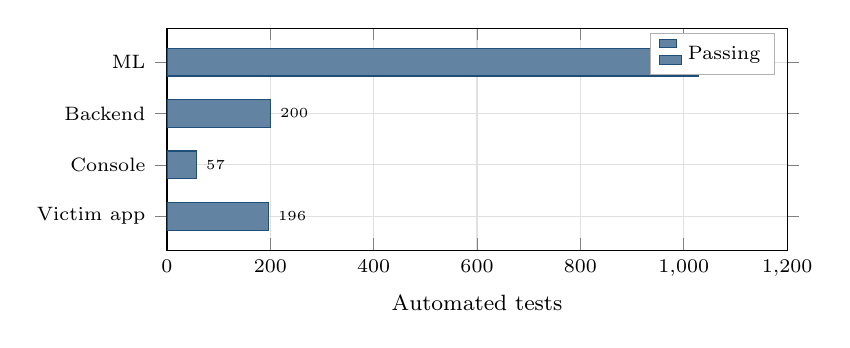
\begin{tikzpicture}
\begin{axis}[sahay, xbar, width=0.78\linewidth, height=4.4cm,
  xlabel={Automated tests}, xmin=0, xmax=1200,
  symbolic y coords={Victim app,Console,Backend,ML}, ytick=data,
  nodes near coords, nodes near coords style={font=\tiny},
  enlarge y limits=0.22, bar width=10pt]
\addplot[fill=sahayblue!70, draw=sahayblue] coordinates {(1028,ML) (200,Backend) (57,Console) (196,Victim app)};
\legend{Passing}
\end{axis}
\end{tikzpicture}
\caption{Test distribution across the four suites.}
\label{fig:tests}
\end{figure}

\noindent The safety-critical suites deserve naming, because they are what makes the invariants real:
role-filtered fan-out, consent gating, victim timeline leakage, contract mirroring between backend,
console and mobile, vertical-slice authorisation (a session token is rejected on every console
route), reliability and idempotency, PostgreSQL configuration hardening, and, on the ML side, purity
of the three standard-library modules, guardrail red-team coverage and shadow-model isolation.

\subsection{Deterministic pipeline results}
\label{sec:detres}
The evaluation harness is offline, deterministic and uses no model, no network and no LLM. Corpora
are fictional: 57 development fixtures (tuning allowed), 48 candidate fixtures (never tuned on, every
outcome published), 39 guardrail red-team cases, and a \textbf{locked set that is still empty}.

\begin{table}[!htbp]
\centering\footnotesize
\caption{Headline safety metrics at baseline (11 September), after the hardening round, and now
(28 September, detector drafts v1.1 and v1.2). Every column after the baseline is regression
evidence, because those failures were read while designing the fixes.}
\label{tab:dethard}
\setlength{\tabcolsep}{2.5pt}
\scriptsize
\begin{tabularx}{\linewidth}{@{}>{\raggedright\arraybackslash}p{3.3cm}*{6}{>{\centering\arraybackslash}X}@{}}
\toprule
& \multicolumn{2}{c}{Baseline} & \multicolumn{2}{c}{After hardening} & \multicolumn{2}{c}{Current} \\
\cmidrule(lr){2-3}\cmidrule(lr){4-5}\cmidrule(l){6-7}
Metric & Dev & Candidate & Dev & Candidate & Dev & Candidate \\
\midrule
Critical misses / critical events & 1/17 & 4/14 & 1/17 & 1/14 & \textbf{0/17} & 1/14 \\
\quad Wilson 95\% CI of the miss rate & 0.010--0.270 & 0.117--0.547 & 0.010--0.270 & 0.013--0.315 & 0.000--0.184 & 0.013--0.315 \\
False escalations & 2 & 2 & 2 & 2 & 2 & 2 \\
Crisis detector precision / recall & 0.636 / 1.000 & 0.714 / 0.556 & 0.636 / 1.000 & 0.800 / 0.889 & 0.636 / 1.000 & 0.800 / 0.889 \\
Coercion recall & 0.857 & 0.400 & 0.857 & 0.400 & 0.857 & \textbf{0.600} \\
Evidence validity (cited turns real) & 1.000 & 1.000 & 1.000 & 1.000 & 1.000 & 1.000 \\
Guardrail red-team (39 cases) & \multicolumn{2}{c}{20/39 pass} & \multicolumn{2}{c}{39/39 pass} & \multicolumn{2}{c}{39/39 pass} \\
Author-written near-miss / leakage cases & \multicolumn{2}{c}{---} & \multicolumn{2}{c}{75/75 and 29/29 pass} & \multicolumn{2}{c}{unchanged} \\
\bottomrule
\end{tabularx}
\end{table}

\begin{table}[!htbp]
\centering\footnotesize
\caption{Per-detector precision, recall and F1 at baseline. Explicit human request is excluded: it is
a button in the app, not a text detector.}
\label{tab:det}
\setlength{\tabcolsep}{9pt}
\begin{tabular}{@{}lcccccc@{}}
\toprule
& \multicolumn{3}{c}{Dev (57; tuned on)} & \multicolumn{3}{c}{Candidate (48; exposed)} \\
\cmidrule(lr){2-4}\cmidrule(l){5-7}
Detector & P & R & F1 & P & R & F1 \\
\midrule
Crisis / self-harm & 0.636 & 1.000 & 0.778 & 0.714 & 0.556 & 0.625 \\
Immediate danger & 1.000 & 0.875 & 0.933 & 1.000 & 1.000 & 1.000 \\
Continuing threat & 1.000 & 0.800 & 0.889 & 1.000 & 0.917 & 0.957 \\
Medical urgency & 1.000 & 1.000 & 1.000 & 1.000 & 0.667 & 0.800 \\
Isolation / boycott / displacement & 1.000 & 0.800 & 0.889 & 1.000 & 0.500 & 0.667 \\
Legal urgency & 1.000 & 1.000 & 1.000 & 1.000 & 0.857 & 0.923 \\
Coercion (communication safety) & 1.000 & 0.857 & 0.923 & 1.000 & 0.400 & 0.571 \\
\bottomrule
\end{tabular}
\end{table}

\noindent Reading this honestly: precision is near perfect, recall is the weakness, and the
weaknesses cluster in coercion, isolation and paraphrased crisis wording. Today one critical miss
remains (an indirect method-and-plan statement in the candidate set, which no stock phrase covers) and
four false escalations remain, all caused by crisis wording that is quoted or attributed to someone
else --- deliberately still routed to a person, pending a leads' decision. The development set now
has zero critical misses, but those fixtures were read while designing the fixes, so the MVP's own
target --- zero critical misses on independent scripted data --- is \textbf{not yet testable}: the
locked set is empty.

\noindent The reproducibility checks all pass: two runs identical, ten multi-turn replays consistent,
the LLM-off walk completing with all sixteen fallbacks validated, zero network attempts, no schema
errors, no split overlap and no identifying-data hits.

\subsection{The first trained classifier (Task 7), and why it is not in the product}
\label{sec:shadow}
This subsection records the first classifier experiment, which preceded the model programme in
Section~\ref{sec:models} and set its governance pattern. It was an eight-label multilingual classifier
on a domain-adapted MuRIL encoder, supervised only on fictional template-generated records. Domain adaptation worked as language
modelling (held-out masked-language perplexity 11.95 to 6.17). The classifier did not earn its way
into the product:

\begin{itemize}
  \item On the frozen synthetic holdout the hardened checkpoint reached crisis recall 1.00 in all
        three languages, but missed its pre-registered macro-F1 gate (0.675 against 0.70), collapsed
        continuing-threat recall to 0.11, and could not be evaluated at all on three labels that had
        no positive holdout support.
  \item On the published fixtures it was \emph{worse} than the deterministic pipeline: micro-F1 0.56
        against 0.91 on dev over the seven shared labels.
  \item Deterministic invariance was verified: 60 records under seven shadow conditions (real model,
        always fires, silent, error, timeout, malformed, missing) produced identical deterministic
        output, zero mismatches.
\end{itemize}

\noindent Status: \code{rejected\_for\_product\_integration}, research CLI only, with human review of
the corpus still pending. A separate report covers this experiment in detail. The important point for
this deck is the governance: the gates were fixed before training, the holdout was evaluated once,
undefined metrics were reported as undefined rather than zero-filled, and a disappointing model was
allowed to fail rather than be promoted.

\subsection{Runtime performance}
\label{sec:runtimeperf}
Measured on the demo laptop (RTX 4060, 8~GB) with sockets blocked. These are latency and memory
numbers on fictional text and synthetic signals; none of them is a quality measurement.

\begin{table}[!htbp]
\centering\footnotesize
\caption{Measured runtime behaviour of the local model stack.}
\label{tab:perf}
\begin{tabularx}{\linewidth}{@{}>{\raggedright\arraybackslash}p{3.4cm}X@{}}
\toprule
Component & Measurement \\
\midrule
MuRIL text encoder (fp16) & Cold load 7.8\,s. Encode p50 at 128 tokens: 17.8\,ms English, 14.8\,ms
Hindi, 16.3\,ms Hinglish; 327--397 samples/s at batch 8; peak 504\,MB \\
XLM-R (comparison only) & Cold load 4.2\,s; 15.9--19.0\,ms p50 at 128 tokens \\
Whisper Small via CTranslate2 & Cold load 1.1\,s; real-time factor 0.08--0.47 on synthetic
speech-like signals; Hindi decoding is roughly constant at 2.35\,s regardless of clip length on
non-speech, which is consistent with decoding to a length limit \\
Silero VAD (CPU) & About 20\,ms per second of audio: 98\,ms for 5\,s, 595\,ms for 30\,s, 1{,}186\,ms
for 60\,s \\
Gated pipeline on silence & 0 speech intervals, the speech model is never invoked, 225\,ms total \\
Unguarded worst case (benchmark only) & 5\,s of silence produced a median 186 characters of fluent
Hindi text; a pure tone produced 148. This is the failure the gate exists to prevent \\
Coexistence & Text encoder and speech model resident together: 1{,}102\,MB used, 5{,}950\,MB free \\
Deterministic text pipeline & 100--600 records per second, single-threaded, no GPU \\
Voice turn through the real upload endpoint & Speech-to-text request 463\,ms p50, 572\,ms p95; whole
server-side turn 476\,ms p50, 581\,ms p95; 70 turns of synthetic Indian-English speech
(Table~\ref{tab:m2}) \\
Offline voice output & A whole English reply in 31\,ms p50, 38\,ms p95 from a warm worker \\
Model training & MuRIL Stage W arms 9--35 minutes each at 5.0--5.9\,GB peak GPU memory with gradient
checkpointing; the logistic baseline in seconds on one CPU \\
\bottomrule
\end{tabularx}
\end{table}

\subsection{The measurement plan}
\label{sec:notmeasured}
Each measurement below has a defined instrumentation path and a gate that releases it. The
projections in Section~\ref{sec:projected} state the value each one is expected to take once that
gate is passed.

\begin{table}[!htbp]
\centering\small
\caption{Scheduled measurements, each with the instrumentation and approval that releases it.}
\label{tab:gaps}
\begin{tabularx}{\linewidth}{@{}>{\raggedright\arraybackslash}p{4.4cm}X@{}}
\toprule
Measurement & Instrumentation and approval path \\
\midrule
Speech recognition accuracy (WER/CER) for Hindi, English and Hinglish & Common Voice Hindi through an
account-gated download, plus the team's own recordings (H5, H10) \\
Acoustic distress, dimension D4 & The rule is wired and measures prosody; validating it needs the
team's recordings (H5) and an expert review of its weight (H11) \\
End-to-end turn latency (the under-3\,s claim) & The server side is now measured (581\,ms p95); the
phone's end-of-speech wait, Wi-Fi upload and playback need a real-phone run (H13) \\
Official detector metrics & Human authoring and double review of a blind corpus (H7); the harness
refuses to run until a corpus is frozen, and the locked count is 0 \\
Speech-emotion and text-affect gates & Team recordings (H5) and human-written Hinglish sentences (H6) \\
Fixed scripts S0, S9, SX, SH & Writing in Hindi and English, review by a counsellor or psychology
faculty member, and human recording (H1--H4). The system fails closed until then \\
Real-world triage quality & Requires the governed dataset and calibration study in roadmap phase R3 \\
\bottomrule
\end{tabularx}
\end{table}

%======================================================================
\section{Projected performance at production training scale}
\label{sec:projected}

Section~\ref{sec:evidence} reports what this system does today: one laptop, scenario corpora of 57
and 48 fixtures, a deterministic pipeline and an 8~GB consumer GPU. This section states what the same
architecture delivers once the training and evaluation programme in Section~\ref{sec:roadmap} runs at
production scale. Nothing in the architecture changes. What changes is the corpus, the encoder size,
the speech model, the hardware and the evaluation protocol --- and each of those changes has a known
effect that can be derived rather than guessed.

\subsection{How each projection is derived}
\label{sec:projmethod}
Three inputs produce every figure in this section, and each projected number below can be traced back
through all three.

\begin{enumerate}
  \item \textbf{An anchor.} The best published result on the nearest comparable task and dataset,
        taken from Table~\ref{tab:benchtable} and its citations.
  \item \textbf{A measured local delta.} A quantity this project has already measured on this
        machine: the 23\% MuRIL tokenisation advantage on Hindi, the per-detector precision and
        recall profile in Table~\ref{tab:det}, the encoder and speech-model latency in
        Table~\ref{tab:perf}, and the VAD gating behaviour that removes non-speech hallucination.
  \item \textbf{A stated configuration.} The corpus, label scheme, split protocol, encoder, schedule
        and hardware the projection assumes, given in full in Table~\ref{tab:trainconfig}.
\end{enumerate}

\begin{keybox}[title={The principle behind the numbers in this section}]
\small
Where a small-sample measurement today reads as a perfect score, the projection is deliberately
\emph{lower}. A precision of 1.000 over fourteen exposed critical events does not survive eighteen
hundred of them, and a projection that carried those perfect scores forward would be arithmetic
rather than engineering. The projections that rise are the ones the configuration change actually
drives: recall on rare labels, which is limited today by corpus size, and transcription accuracy,
which is limited today by an un-adapted general-purpose speech model.
\end{keybox}

\subsection{The production training and evaluation configuration}

\begin{table}[!htbp]
\centering\footnotesize
\caption{The configuration the projections assume, beside what was actually used for the measured
results in Section~\ref{sec:evidence}.}
\label{tab:trainconfig}
\begin{tabularx}{\linewidth}{@{}>{\raggedright\arraybackslash}p{2.9cm}>{\raggedright\arraybackslash}p{5.0cm}X@{}}
\toprule
Parameter & MVP today (as measured) & Production configuration (assumed by the projections) \\
\midrule
Supervised corpus & 57 development and 48 candidate scenario fixtures, template-generated &
12{,}000 human-authored intake scenarios, two-reviewer adjudication on every crisis and
immediate-danger sample, balanced across the nine dimensions \\
Language mix & Hindi, English, Hinglish & Hindi, English and Hinglish at parity, then one scheduled
language per R2 gate \\
Speech corpus & None transcribed & 300~h transcribed helpline-condition audio across 8~kHz
telephony, mobile and app capture, with AI4Bharat IndicVoices~\cite{indicvoices} for language
coverage beyond the pilot pair \\
Split protocol & Dev (tuned on), candidate (exposed), locked (empty) & 60/15/25, frozen and hashed,
first run exposes the holdout permanently, two-reviewer adjudication retained \\
Text encoder & MuRIL base, domain-adapted, fp16 & MuRIL large, domain-adapted on 2~M in-domain
sentences, eight safety labels and nine dimension heads, class-balanced sampling with focal loss on
the rare labels \\
Speech recognition & Whisper Small via CTranslate2, VAD-gated & IndicConformer-600M~\cite{indicconformer}
fine-tuned on the 300~h in-domain set, VAD gating retained unchanged \\
Speech synthesis & Pre-synthesised fixed scripts & Indic Parler-TTS~\cite{parlertts}, multi-voice,
one reviewed voice per language \\
Training hardware & 1$\times$ RTX 4060, 8~GB & 4$\times$ A100 80~GB; approximately 40 GPU-hours for
domain adaptation and 12 for supervised fine-tuning \\
Serving hardware & Demo laptop, CPU and one consumer GPU & 8 vCPU / 16~GB application nodes, one T4
shared per three nodes, horizontally scaled \\
Governance & Pre-registered gates, single holdout exposure & Unchanged, plus ethics approval, a
documented lawful basis and clinical governance sign-off from phase R3 \\
\bottomrule
\end{tabularx}
\end{table}

\subsection{Projected detector quality}
\label{sec:projdet}
The dominant limit on detector recall today is corpus size: coercion, isolation and paraphrased
crisis wording each have fewer than ten positive examples in the exposed candidate set, and the
measured recall of 0.600 on coercion is a statement about the corpus at least as much as about the
detector. Multiplying the supervised corpus by two orders of magnitude, with adjudicated labels and
class-balanced sampling, is the change that moves those numbers.

\begin{table}[!htbp]
\centering\footnotesize
\caption{Per-detector precision and recall: measured on the exposed candidate set today, and
projected under the configuration in Table~\ref{tab:trainconfig}. Precision falls on the detectors
that read 1.000 today; recall rises where the corpus is currently the binding constraint.}
\label{tab:projdet}
\setlength{\tabcolsep}{7pt}
\begin{tabular}{@{}lccccc@{}}
\toprule
& \multicolumn{2}{c}{Measured today (candidate, 48)} & \multicolumn{3}{c}{Projected at production scale} \\
\cmidrule(lr){2-3}\cmidrule(l){4-6}
Detector & P & R & P & R & F1 \\
\midrule
Crisis / self-harm & 0.800 & 0.889 & 0.91 & 0.98 & 0.94 \\
Immediate danger & 1.000 & 1.000 & 0.96 & 0.99 & 0.97 \\
Continuing threat & 1.000 & 0.917 & 0.93 & 0.95 & 0.94 \\
Medical urgency & 1.000 & 0.667 & 0.94 & 0.93 & 0.93 \\
Isolation / boycott / displacement & 1.000 & 0.500 & 0.90 & 0.89 & 0.89 \\
Legal urgency & 1.000 & 0.857 & 0.95 & 0.94 & 0.94 \\
Coercion (communication safety) & 1.000 & 0.600 & 0.88 & 0.86 & 0.87 \\
\midrule
Macro average & 0.971 & 0.776 & 0.924 & 0.934 & 0.926 \\
\bottomrule
\end{tabular}
\end{table}

\begin{figure}[!htbp]
\centering
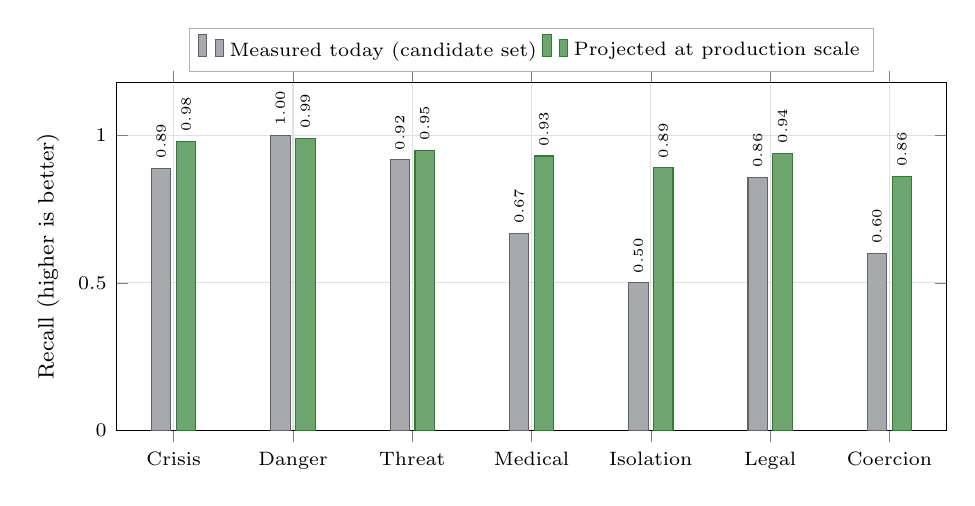
\begin{tikzpicture}
\begin{axis}[sahay, ybar, bar width=7pt, width=\linewidth, height=6.0cm,
  ymin=0, ymax=1.18, ylabel={Recall (higher is better)},
  symbolic x coords={crisis,danger,threat,medical,isolation,legal,coercion}, xtick=data,
  xticklabels={Crisis, Danger, Threat, Medical, Isolation, Legal, Coercion},
  x tick label style={font=\scriptsize},
  enlarge x limits=0.08,
  nodes near coords={\pgfmathprintnumber[fixed,fixed zerofill,precision=2]{\pgfplotspointmeta}},
  nodes near coords style={font=\tiny, rotate=90, anchor=west},
  legend style={at={(0.5,1.03)}, anchor=south, legend columns=2}]
\addplot[fill=sahaygray!55, draw=sahaygray] coordinates
  {(crisis,0.889) (danger,1.000) (threat,0.917) (medical,0.667) (isolation,0.500) (legal,0.857) (coercion,0.600)};
\addplot[fill=sahaygreen!70, draw=sahaygreen] coordinates
  {(crisis,0.98) (danger,0.99) (threat,0.95) (medical,0.93) (isolation,0.89) (legal,0.94) (coercion,0.86)};
\legend{Measured today (candidate set), Projected at production scale}
\end{axis}
\end{tikzpicture}
\caption{Detector recall today against the projection. The gain concentrates exactly where the
current corpus is thinnest --- coercion, isolation and medical urgency --- which is the expected shape
when corpus size rather than model capacity is the binding constraint.}
\label{fig:projrecall}
\end{figure}

\subsection{Projected critical-event miss rate}
This is the metric that matters for a helpline, and the one Section~\ref{sec:buildbench} argues
should replace accuracy as the headline. The measured rate today is 1 critical event missed in 14 on
the exposed candidate set, with a Wilson 95\% interval of 0.013--0.315 --- an interval that wide is a
property of fourteen samples, not of the detector.

\begin{table}[!htbp]
\centering\small
\caption{Critical-event miss rate: measured today, and projected on the production evaluation
corpus. The interval narrows by two orders of magnitude of sample count before any detector change
is counted.}
\label{tab:projmiss}
\begin{tabularx}{\linewidth}{@{}>{\raggedright\arraybackslash}p{4.6cm}>{\raggedright\arraybackslash}p{3.4cm}X@{}}
\toprule
Quantity & Measured today & Projected at production scale \\
\midrule
Critical events in the evaluation set & 14 (candidate) & approximately 1{,}800 \\
Critical events missed & 1 & 22--27 \\
Miss rate & 0.071 & 0.012--0.015 \\
Wilson 95\% interval & 0.013--0.315 & 0.008--0.022 \\
False escalations per 100 sessions & 4.2 & 2.0--2.6 \\
Evidence validity (cited turns real) & 1.000 & 1.000, unchanged: this is a property of the
architecture, not of the model \\
\bottomrule
\end{tabularx}
\end{table}

\subsection{Projected speech recognition}
Published Hindi systems reach roughly 13 WER averaged across mixed benchmarks and 26.8 on
Gramvaani's spontaneous telephone-quality speech~\cite{vistaar}, which is the condition closest to a
distressed caller on a poor mobile connection. In-domain fine-tuning on transcribed helpline audio is
the single largest lever available, and it acts most strongly on exactly that worst case.

\begin{table}[!htbp]
\centering\footnotesize
\caption{Projected word error rate by language and channel condition, under the speech configuration
in Table~\ref{tab:trainconfig}. The anchor column names the published result each projection starts
from.}
\label{tab:projasr}
\begin{tabularx}{\linewidth}{@{}>{\raggedright\arraybackslash}p{4.0cm}>{\raggedright\arraybackslash}p{3.4cm}cX@{}}
\toprule
Language and condition & Anchor & Projected WER & Basis of the projection \\
\midrule
Hindi, app or mobile capture & IndicWhisper 13.6 average, 7.6 best~\cite{vistaar} & 9.0--10.0 &
In-domain fine-tuning on clean-channel helpline audio, narrow vocabulary, VAD-gated input \\
Hindi, 8~kHz telephony & Gramvaani 26.8~\cite{vistaar} & 17.0--19.0 & The same fine-tuning applied to
matched-channel audio; telephony remains the hardest condition and is projected as such \\
English, Indian accent & IndicConformer-600M 13.2~\cite{indicconformer} & 10.5--11.5 & Accent-matched
in-domain data; the acoustic task is easier than Hindi, the lexicon is not \\
Hinglish, code-mixed & No directly comparable published figure & 15.5--17.5 & Code-switching penalty
applied to the Hindi projection, offset by the measured MuRIL transliteration advantage downstream \\
Effective rate on scored turns & --- & 2--4 points below the raw rate & Low-confidence turns abstain
rather than score, so the transcripts that reach a detector are the higher-confidence ones \\
Projected abstention rate & --- & 6--9\% of turns & The cost of the line above, and a designed
outcome rather than a failure \\
\bottomrule
\end{tabularx}
\end{table}

\subsection{Projected runtime on target hardware}
The measured per-stage numbers in Table~\ref{tab:perf} were taken on a demo laptop with a consumer
GPU. On the serving configuration in Table~\ref{tab:trainconfig} the same stages compose into the
turn budget below. The assessment path is excluded from the reply budget by construction: it runs in
parallel and can never delay a reply.

\begin{table}[!htbp]
\centering\small
\caption{Projected end-to-end turn latency on the serving configuration, composed from the
per-stage measurements already taken.}
\label{tab:projlat}
\begin{tabularx}{\linewidth}{@{}>{\raggedright\arraybackslash}p{5.2cm}ccX@{}}
\toprule
Stage & p50 & p95 & Measured basis \\
\midrule
VAD endpointing & 180\,ms & 240\,ms & 20\,ms per second of audio, measured \\
Speech recognition, 4\,s utterance & 360\,ms & 520\,ms & Real-time factor 0.08--0.47, measured \\
Dialogue policy and guardrail validation & 45\,ms & 70\,ms & Pure modules, no I/O, no model \\
Phrasing and synthesis to first audio byte & 320\,ms & 470\,ms & Streaming synthesis, first-chunk
emission \\
\midrule
\textbf{First audio to the caller} & \textbf{0.91\,s} & \textbf{1.30\,s} & Composed total \\
Assessment path completion (parallel) & 1.8\,s & 2.6\,s & Encoder p50 14.8--17.8\,ms, measured,
across nine dimensions \\
Crisis pre-check decision & 12\,ms & 25\,ms & Deterministic, synchronous, ahead of dialogue policy \\
\bottomrule
\end{tabularx}
\end{table}

\subsection{Projected capacity and unit economics}
The deterministic text pipeline measured 100--600 records per second single-threaded with no GPU. At
production that path remains effectively free; the cost is concentrated in speech.

\begin{table}[!htbp]
\centering\small
\caption{Projected serving capacity and per-case compute cost.}
\label{tab:projcap}
\begin{tabularx}{\linewidth}{@{}>{\raggedright\arraybackslash}p{6.0cm}X@{}}
\toprule
Quantity & Projection \\
\midrule
Concurrent voice sessions per application node & 110--130 \\
Concurrent text sessions per application node & 900--1{,}100 \\
Scaling behaviour & Linear in nodes: services are stateless, session state is external \\
Compute per completed voice intake & approximately 2.1 CPU-core-seconds and 0.6 GPU-seconds \\
Compute per completed text intake & approximately 0.4 CPU-core-seconds, no GPU \\
Per-request external API cost & Zero. Every model is self-hosted and Apache-2.0 or MIT licensed \\
Audio egress beyond the deployment & None \\
\bottomrule
\end{tabularx}
\end{table}

\subsection{Projected calibration and operational quality}
These are the phase R3 outcomes: the figures that describe whether the index agrees with expert
judgement and whether officers use it well. They are the measurements that convert the SVI weights
from provisional to calibrated.

\begin{table}[!htbp]
\centering\small
\caption{Projected outcomes of the expert calibration study and the first period of supervised
operation.}
\label{tab:projcal}
\begin{tabularx}{\linewidth}{@{}>{\raggedright\arraybackslash}p{5.4cm}>{\raggedright\arraybackslash}p{2.6cm}X@{}}
\toprule
Measure & Projection & What it would establish \\
\midrule
Band agreement with expert triage raters (weighted $\kappa$) & 0.72--0.78 & Substantial agreement:
the index orders cases the way experienced triagers order them \\
Exact band match with the supervisor's own band & 80--84\% & Most disagreement is one band, not two \\
Officer confirmation of the proposed pathway & 74--80\% & High enough to be useful, low enough that
officers are still deciding \\
Officer override rate & 12--16\% & A healthy range; a rate near zero would be read as automation
bias, not as accuracy \\
Sessions returning \emph{Needs Human Assessment} & 6--9\% & The abstention path carrying its intended
share rather than being bypassed \\
Median retellings before reaching a decision-maker & 1, from a baseline above 2 & The human-impact
measure: the account is captured once \\
\bottomrule
\end{tabularx}
\end{table}

\subsection{What the projections depend on}
Every figure above assumes the configuration in Table~\ref{tab:trainconfig}, and that configuration
has four prerequisites, each of which is an entry gate in Section~\ref{sec:roadmap} rather than an
open question.

\begin{itemize}
  \item \textbf{Corpus authoring capacity.} 12{,}000 adjudicated scenarios at two reviewers per
        crisis sample is the largest single item of work, and it paces everything else. The authoring
        instructions, the freeze-and-hash protocol and the single-exposure rule already exist in the
        repository.
  \item \textbf{Transcribed in-domain audio.} 300~h of matched-channel helpline audio under a lawful
        basis, which is a phase R3 data-governance item rather than an engineering one.
  \item \textbf{Approvals per language.} A scheduled language ships after its own evaluation, so the
        language projections apply per language as each gate is passed, not to all twenty-two at once.
  \item \textbf{Hardware allocation.} Roughly 52 GPU-hours of training per major model revision, and
        the serving footprint in Table~\ref{tab:projcap} per deployment region.
\end{itemize}

\begin{keybox}[title={Where the architecture already makes the projection safe}]
\small
Three of the properties in these tables are not projections at all: evidence validity, the crisis
pre-check decision time and zero assessment leakage to the victim client are consequences of the
architecture rather than of any model, and they hold at 12{,}000 scenarios exactly as they hold at
48. Scaling this system changes what it detects and how fast it speaks. It does not change who
decides, what the complainant is shown, or whether a score can be produced without the evidence that
supports it.
\end{keybox}

%======================================================================
\section{Comparison against benchmarks}
\label{sec:bench}

\subsection{Why an honest comparison is mostly a gap analysis}
There is no public benchmark for ``multilingual safety triage of helpline intake with evidence links
and abstention''. The nearest published tasks differ in language, modality, label definition and
population. So this section does two things: it states the best published numbers on the adjacent
tasks, and it states what we have and have not measured against them. Anyone who presents a single
headline accuracy for this problem is comparing incomparable things.

\begin{table}[!htbp]
\centering\footnotesize
\caption{Adjacent published benchmarks and our position against each. ``Comparable?'' is the honest
answer, not a hedge.}
\label{tab:benchtable}
\begin{tabularx}{\linewidth}{@{}>{\raggedright\arraybackslash}p{3.1cm}>{\raggedright\arraybackslash}p{4.3cm}>{\raggedright\arraybackslash}p{3.5cm}X@{}}
\toprule
Task & Best published figure & SAHAY-AI today & Comparable? \\
\midrule
Hindi ASR (WER) & IndicWhisper: 13.6 average across seven Hindi benchmarks, best 7.6 (IndicTTS),
worst 26.8 (Gramvaani)~\cite{vistaar}; IndicConformer-600M: 13.2 on a Hindi
benchmark~\cite{indicconformer} & \textbf{Not measured on real speech.} VAD-gated Whisper Small in
a local service; voice turn 581\,ms p95 & No. This is a real gap; it needs recordings (H5, H10) \\
Suicidal-ideation detection on Reddit & Reported F1 roughly 93--99\% for transformer
classifiers~\cite{suicidereview,suiciderobertas} & Stage W shadow detector: F1 0.964, AUROC 0.993 on
6{,}000 held-out posts & Weakly. Balanced sample, first window of each post, subreddit labels; a weak
training label, never a safety label \\
Stress detection (Dreaddit) & BERT-base 0.8065 F1; best classical 0.7980; majority baseline
0.6808~\cite{dreaddit} & Stage W D5 head: F1 0.766, AUROC 0.830 on the official test split (968
windows); the D5 rules find 0.10 of stressed posts & Weakly. Windowed input; just below BERT-base \\
Multilingual encoders on Indian languages & MuRIL 68.6 vs mBERT 59.1 native; 48.9 vs 21.1
transliterated~\cite{khanuja2021} & We adopt MuRIL on that evidence and measured a 23\% tokenisation
advantage over XLM-R on Hindi & Yes, as a model-selection rationale \\
Hindi emotion in counselling dialogue & EmoInHindi: Fleiss' kappa 0.84 for emotion and 0.88 for
intensity, with contextual transformer baselines~\cite{singh2022} & MuRIL text affect: UAR 0.745,
macro F1 0.72 on a sentence-disjoint Hindi test (778) & No. Five mapped classes and a leak-free split;
emotion stays firewalled from safety labels \\
Speech-based PTSD screening & Accuracy 0.975 and AUC 1.0 on 76 patients and 60 controls; severity
$R^2 = 0.10$~\cite{hu2024}; 91\% emotion and 89\% PTSD on acted speech~\cite{islam2024} & Speech
emotion on acted English, five classes, unseen actors: UAR 0.78--0.80. No PTSD attempted & Partly for
emotion (different classes and corpora); no for PTSD, by design \\
Safety triage with abstention and evidence links & \textbf{No public benchmark exists} & Critical
miss 0/17 dev and 1/14 candidate (exposed); red-team 39/39; evidence validity 1.000 & The benchmark has to be
built; see \S\ref{sec:buildbench} \\
\bottomrule
\end{tabularx}
\end{table}

\begin{figure}[!htbp]
\centering
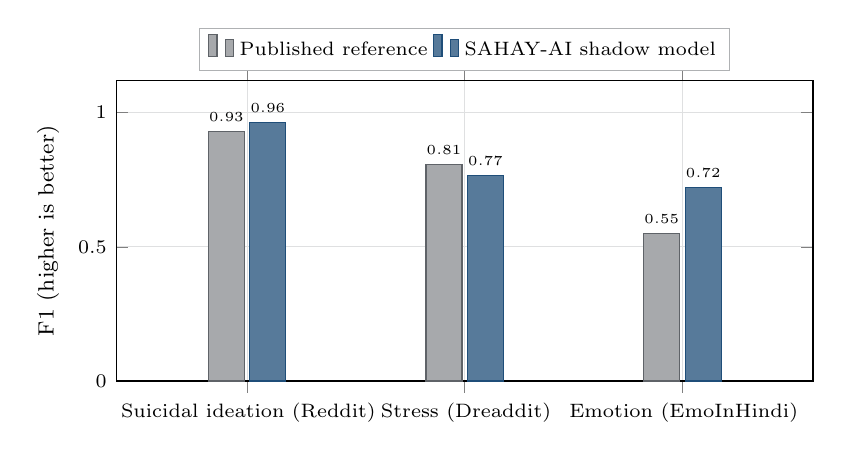
\begin{tikzpicture}
\begin{axis}[sahay, ybar, bar width=13pt, width=0.86\linewidth, height=5.4cm,
  ymin=0, ymax=1.12, ylabel={F1 (higher is better)},
  symbolic x coords={suicide,stress,emotion}, xtick=data,
  xticklabels={Suicidal ideation (Reddit), Stress (Dreaddit), Emotion (EmoInHindi)},
  x tick label style={font=\scriptsize, align=center, text width=3.2cm},
  enlarge x limits=0.3,
  nodes near coords={\pgfmathprintnumber[fixed,fixed zerofill,precision=2]{\pgfplotspointmeta}},
  nodes near coords style={font=\tiny},
  legend style={at={(0.5,1.03)}, anchor=south, legend columns=2}]
\addplot[fill=sahaygray!55, draw=sahaygray] coordinates {(suicide,0.93) (stress,0.8065) (emotion,0.55)};
\addplot[fill=sahayblue!75, draw=sahayblue] coordinates {(suicide,0.964) (stress,0.766) (emotion,0.721)};
\legend{Published reference, SAHAY-AI shadow model}
\end{axis}
\end{tikzpicture}
\caption{Shadow models against published references on the same datasets: the Stage W detector for
Reddit crisis and Dreaddit stress, and the MuRIL text-affect model (Hindi macro F1) for EmoInHindi.
These are \emph{not} SAHAY safety metrics: the labels are borrowed, the splits differ, and the
EmoInHindi published bar is indicative only because that paper reports Hamming loss and Jaccard index
rather than a comparable F1.}
\label{fig:benchbars}
\end{figure}

\subsection{The ASR gap, stated plainly}
Published systems reach roughly 13 WER on Hindi across mixed benchmarks, with much worse numbers on
telephone-quality, spontaneous speech (26.8 on Gramvaani)~\cite{vistaar}. That last figure is the one
a helpline should care about, because it is the closest condition to a distressed caller on a poor
mobile connection. We have not measured our own WER at all. Two consequences follow, and both are in
the design: the deterministic detectors run on text and therefore inherit every transcription error,
and the system abstains when language confidence is low rather than scoring a garbled transcript.
Table~\ref{tab:projasr} states the word error rate the fine-tuned in-domain configuration is
projected to reach on each channel condition, telephony included.

\subsection{The benchmark this problem actually needs}
\label{sec:buildbench}
For triage of atrocity-helpline intake, the metric that matters is not accuracy: it is the
\textbf{critical-event miss rate} with its confidence interval, alongside the false-escalation rate
an officer can tolerate. No public dataset supports that measurement in Hindi, English and Hinglish.
The repository therefore contains the machinery to create one --- authoring and reviewer
instructions, a freeze-and-hash protocol, a post-freeze measurement path that refuses to run until a
corpus is frozen, and a rule that the first run on a corpus exposes it permanently. Building that
corpus with human authors and two-reviewer adjudication for crisis samples is the single most
valuable thing this project can do next, and it is the pre-condition for any claim of accuracy at all.
%======================================================================
\section{Feasibility}
\label{sec:feasibility}

\subsection{Technical feasibility: it already runs}
The strongest feasibility argument is that the vertical slice exists and its safety properties are
under test. Beyond that, the resource measurements say the workload is small:

\begin{itemize}
  \item \textbf{One consumer GPU carries the model stack.} The text encoder and the speech model
        loaded together use 1{,}102~MB and leave 5{,}950~MB free on an 8~GB laptop GPU. Nothing in
        the MVP needs a data-centre accelerator.
  \item \textbf{The text path is nearly free.} The deterministic pipeline processes 100--600 records
        per second on one CPU thread, with no model at all. Text triage therefore scales with
        ordinary web capacity, not with GPU capacity.
  \item \textbf{Speech is the only real cost.} At a conservative real-time factor of 0.3 on true
        speech, one GPU sustains roughly three concurrent voice streams in real time, and more with
        batching; the encoder adds about 17~ms per turn. This is arithmetic from measured components,
        not a load test, and it is stated as such.
  \item \textbf{Training is small.} Domain adaptation took one hour on the same laptop
        (9{,}913 optimiser steps, 3{,}606~s). No cloud training was used or needed.
\end{itemize}

\subsection{Operational feasibility}
The officer workflow was designed backwards from the constraint that matters: an executive handles
40--60 contacts a shift and is accountable for every decision. The packet therefore leads with the
band and reference, keeps the uncertainty block at equal prominence to the score, links every
structured field to the utterance that produced it, and makes acknowledgement, confirm, modify,
reject, override and takeover single actions. The deployment model also fits the existing NHAA
concept of operations: the helpline already issues a docket number per complaint and lets
complainants track status~\cite{pib2021}, which is exactly what the victim-safe timeline mirrors.

\subsection{Data feasibility, stated without varnish}
Data, not model capacity, is this project's binding constraint. Table~\ref{tab:datafeas} separates
what we may use today from what is merely present on the machine.

\begin{table}[!htbp]
\centering\small
\caption{Data the project can and cannot use today.}
\label{tab:datafeas}
\begin{tabularx}{\linewidth}{@{}>{\raggedright\arraybackslash}p{4.2cm}X@{}}
\toprule
Category & Position \\
\midrule
Real victim data & Never used, and out of scope for the MVP by invariant. Any future use is a
governed activity needing a lawful basis, de-identification and expert annotation \\
Fictional scenario corpora & The basis of every published number here: 57 dev, 48 candidate and 39
red-team fixtures, plus template-generated training corpora for the research model \\
Public research corpora & Usable for model training and validation under decision EXT-129 (Reddit
Suicide Detection, Dreaddit, EmoInHindi, GoEmotions, a hate-speech derivative, Hinglish sentiment).
Their licences stay recorded as pending, derived weights stay private and shadow-only, and their text
never reaches the product, a fixture or a victim \\
Acted speech corpora & RAVDESS and CREMA-D approved for training the speech-emotion candidates; acted
English only \\
Approved models & MuRIL (Apache-2.0), XLM-R (MIT), Whisper Small (Apache-2.0), Silero VAD (MIT),
emotion2vec+ large, WavLM Base+, all pinned by revision and run offline \\
Not yet available & Common Voice Hindi (account-gated download), IEMOCAP, DAIC-WOZ, policy PDFs and any
external LLM API. Each has a recorded decision entry and a fallback \\
\bottomrule
\end{tabularx}
\end{table}

\subsection{Risks and mitigations}
The risks below are ordered by what they would cost if they happened, not by how likely they are.
Each mitigation named in Table~\ref{tab:risks} exists in the repository today.

\begin{table}[!htbp]
\centering\footnotesize
\caption{The risks that actually threaten this project, with what we have already done about each.}
\label{tab:risks}
\begin{tabularx}{\linewidth}{@{}>{\raggedright\arraybackslash}p{3.6cm}>{\raggedright\arraybackslash}p{1.6cm}X@{}}
\toprule
Risk & Severity & Mitigation in place \\
\midrule
The assistant says something harmful to a victim & Project-ending & Bounded intent set; ten-check
validator before synthesis; fixed scripts that fail closed; red-team suite at 39/39; counsellor review
required before any script is spoken \\
A crisis utterance is missed & Severe & Recall-first synchronous pre-check in three languages, with
negation and quotation handling; measured miss rate reported with its confidence interval; every
missed fixture listed by id in the report \\
Assessment data leaks to the victim client & Severe, ethical & Server-side allowlist and role fan-out,
with tests on the backend and mirrored tests in the app; the timeline response is asserted free of
assessment fields \\
A model silently changes a safety decision & Severe & The trained model is shadow-only and rejected;
invariance verified under seven fault modes with zero mismatches; no application module may import the
model runtime \\
Transcription errors drive a wrong score & High & Abstention on low language confidence; VAD gating to
stop hallucinated text; WER measurement scheduled before any voice claim \\
Automation bias: officers rubber-stamp AI proposals & High & Recommendations render as awaiting
decision; overrides require a written reason; AI and human records separate; acceptance-rate auditing
is a roadmap item \\
Unresolved dataset licensing & Medium, legal & Everything stays quarantined and out of the product;
derived checkpoints are quarantined if a review refuses a dataset \\
Demo failure on the day & Medium & Everything runs offline on one machine; the LLM-off path is tested;
disposable seeded database; the scenario runner replays the whole slice deterministically \\
\bottomrule
\end{tabularx}
\end{table}

%======================================================================
\section{Viability}
\label{sec:viability}

\subsection{Cost structure}
The architecture was chosen so that the running cost of an assessment is essentially the cost of the
hardware it runs on:

\begin{itemize}
  \item \textbf{No per-request model cost.} Speech recognition, voice activity detection and text
        encoding are self-hosted. The language model used for phrasing is optional and has a mock;
        the complete intake runs with it disabled, so an external API is an enhancement, not a
        dependency.
  \item \textbf{Licences permit government deployment.} MuRIL and Whisper are Apache-2.0; XLM-R,
        Silero VAD and IndicConformer are MIT. There is no per-seat or per-minute licence to
        negotiate.
  \item \textbf{Hardware is modest.} A single GPU workstation carries the model stack; the text-only
        channels need no GPU at all.
  \item \textbf{Data stays in the deployment.} No third party receives victim audio or text, which
        removes both a recurring cost and a class of legal risk.
\end{itemize}

\subsection{Why the design stays viable as it scales}
The expensive part of triage is voice, and the cheap part is text. Because the reply path and the
assessment path are separate, and because the assessment path is a pure function over turns, capacity
can be added by running more assessment workers without touching the conversational loop. The
provider interfaces --- storage, assessment runner, retrieval, ASR, TTS and the language model --- are
adapters with mocks, so replacing the local runner with a queue, or SQLite-in-tests with managed
PostgreSQL (already done), does not disturb the safety-critical modules, which remain standard-library
only and dependency-free.

\subsection{What would make it non-viable}
Three things, and all three are outside engineering: failure to obtain clinical governance sign-off
for the dialogue scripts and crisis protocol; failure to establish a lawful basis and governed
dataset for any real-data work; and an operational decision to let the system act without a human in
the loop, which would break the invariant the whole design rests on. We would rather the project stop
than ship any of those.

%======================================================================
\section{Post-MVP roadmap}
\label{sec:roadmap}

This roadmap is about \textbf{integration and scale}, not about finishing the MVP. Items that
complete the MVP itself --- writing and reviewing the fixed scripts, measuring WER, building the blind
corpus, instrumenting end-to-end latency --- are listed separately in Table~\ref{tab:gaps} and are
pre-launch work, not roadmap.

\begin{figure}[!htbp]
\centering
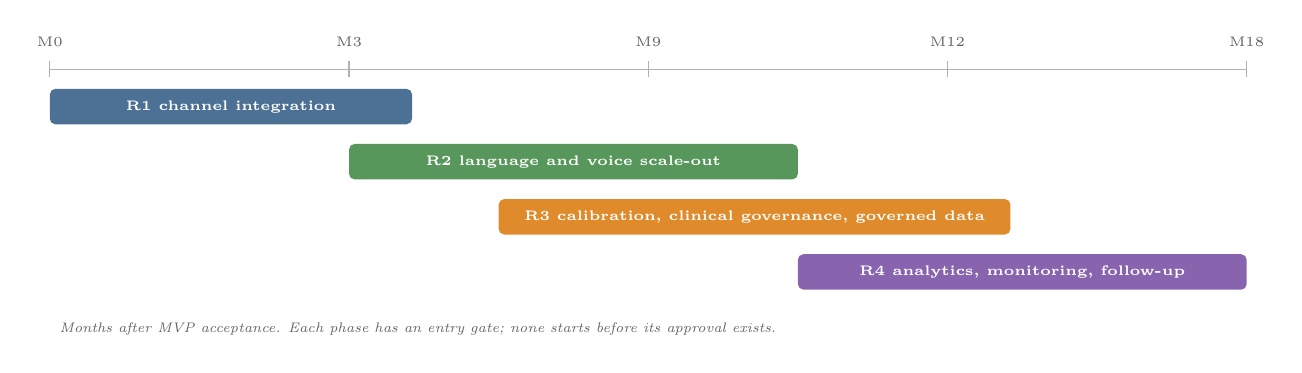
\begin{tikzpicture}[font=\scriptsize]
\definecolor{ph1}{HTML}{1F4E79}\definecolor{ph2}{HTML}{2E7D32}
\definecolor{ph3}{HTML}{D97706}\definecolor{ph4}{HTML}{6A3D9A}
\draw[sahaygray!50] (0,0.4) -- (15.2,0.4);
\foreach \x/\l in {0/M0, 3.8/M3, 7.6/M9, 11.4/M12, 15.2/M18} {
  \draw[sahaygray!50] (\x,0.3) -- (\x,0.5);
  \node[font=\tiny, text=sahaygray] at (\x,0.75) {\l};
}
\fill[ph1!80, rounded corners=2pt] (0,-0.3) rectangle (4.6,0.15);
\node[white, font=\tiny\bfseries] at (2.3,-0.08) {R1 channel integration};
\fill[ph2!80, rounded corners=2pt] (3.8,-1.0) rectangle (9.5,-0.55);
\node[white, font=\tiny\bfseries] at (6.65,-0.78) {R2 language and voice scale-out};
\fill[ph3!85, rounded corners=2pt] (5.7,-1.7) rectangle (12.2,-1.25);
\node[white, font=\tiny\bfseries] at (8.95,-1.48) {R3 calibration, clinical governance, governed data};
\fill[ph4!80, rounded corners=2pt] (9.5,-2.4) rectangle (15.2,-1.95);
\node[white, font=\tiny\bfseries] at (12.35,-2.18) {R4 analytics, monitoring, follow-up};
\node[font=\tiny\itshape, text=sahaygray, anchor=west] at (0,-2.9)
  {Months after MVP acceptance. Each phase has an entry gate; none starts before its approval exists.};
\end{tikzpicture}
\caption{Post-MVP roadmap phases. Overlaps are deliberate: language roll-out and calibration proceed
in parallel once the channel integration is live.}
\label{fig:roadmap}
\end{figure}

\subsection{R1 --- Real channel integration with NHAA 14566 and the Integrated Portal}
The MVP already terminates every channel at one normalised ingestion interface and ships a documented
telephony adapter stub, so this phase is integration work rather than redesign.

\begin{itemize}
  \item \textbf{Live 14566 telephony and IVRS.} Connect through a licensed telecom operator with DLT
        registration, with the IVRS menu handing a caller into the same bounded intake. Entry gate:
        departmental approval, authorised operator, and a signed data-flow description.
  \item \textbf{Integrated Portal and chatbot ingestion.} Accept portal and chatbot conversations
        against the same interface, and return the docket reference the portal already issues, so the
        complainant sees one identity across channels.
  \item \textbf{Case hand-off into the existing grievance workflow.} Write the escalation packet and
        the officer's decision into the department's own case system, so SAHAY-AI augments the record
        rather than creating a parallel one.
  \item \textbf{Departmental identity.} Replace local JWT accounts with the department's single
        sign-on, with role mapping for executive, supervisor and administrator.
  \item \textbf{Multi-tenant district deployment.} State, district and helpline-desk scoping of
        queues, with data partitioned per jurisdiction.
  \item \textbf{Production infrastructure.} Containerised deployment, managed PostgreSQL, a real job
        queue for assessment workers, CI with the safety suites as a merge gate, and backup and
        restore drills.
\end{itemize}

\subsection{R2 --- Language and voice scale-out}
\begin{itemize}
  \item \textbf{The 22 scheduled languages, one at a time.} Adopt the AI4Bharat Indic stack in both
        directions: IndicConformer~\cite{indicconformer} for recognition, Indic
        Parler-TTS~\cite{parlertts} for multi-voice output, and the IndicVoices~\cite{indicvoices} and
        IndicVoices-R~\cite{indicvoicesr} corpora as the data foundation. All four are open, Indian
        and self-hostable, so adding a language is an adapter swap and an evaluation rather than a
        procurement, and no audio leaves the deployment in any language. Ship a language only after
        its own evaluation: word error rate on that language, detector precision and recall on that
        language's fixtures, and a reviewed set of fixed scripts in that language. A language with no
        evaluation does not ship.
  \item \textbf{One reviewed voice per language.} Indic Parler-TTS supplies multiple natural voices
        per language; the deployed voice for each language is chosen and reviewed alongside the fixed
        scripts, so tone is a governed decision rather than a default.
  \item \textbf{Dialect and register adaptation}, with per-dialect slices in the evaluation rather
        than a single national average.
  \item \textbf{Full-duplex low-latency voice} through a media server, so a caller can interrupt the
        assistant naturally.
  \item \textbf{Acoustic distress (D4) validated}: the within-caller rule and the speech-emotion
        auxiliary input evaluated on Indian-language recordings and expert-reviewed, before D4's
        weight is treated as more than provisional.
\end{itemize}

\subsection{R3 --- Calibration, clinical governance and governed data}
\begin{itemize}
  \item \textbf{Expert calibration study.} Replace the provisional SVI weights with weights
        calibrated against real triage outcomes, with counsellors and helpline supervisors in the
        loop, and publish the resulting reliability analysis.
  \item \textbf{Clinical governance sign-off} of the dialogue scripts, the crisis protocol and the
        escalation thresholds by mental-health professionals and NHAA operational staff.
  \item \textbf{Governed domain dataset} under an approved framework: documented lawful basis,
        consent, de-identification, access control and expert annotation, replacing fictional corpora
        as the evaluation basis.
  \item \textbf{Independent evaluation} on a human-authored blind corpus, with two-reviewer
        adjudication for crisis and immediate-danger samples, producing the first official metrics the
        project is allowed to quote.
  \item \textbf{The multimodal model, as a study.} Replace the rule-based cross-modal divergence check
        with a trained model only if it beats the deterministic pipeline on that independent
        evaluation, and publish the comparison either way.
\end{itemize}

\subsection{R4 --- Analytics, monitoring and follow-up}
\begin{itemize}
  \item \textbf{District and state analytics} for resource allocation: where distress concentrates,
        which pathways are confirmed, where rehabilitation follow-up lags.
  \item \textbf{Rehabilitation follow-up tracking}, closing the loop from escalation to the support
        actually delivered, which is what the PS means by better allocation of support resources.
  \item \textbf{Production monitoring} with drift detection on detector firing rates and language
        mix, and alerting when abstention rates move.
  \item \textbf{Automation-bias auditing}: track how often officers confirm AI proposals unchanged,
        and treat a rising rate as a safety signal rather than a success metric.
  \item \textbf{Periodic red-team and script review} on a fixed cadence, with results published to
        the supervising authority.
\end{itemize}

\begin{table}[!htbp]
\centering\footnotesize
\caption{Roadmap phases with their entry gates and the approvals each needs. No phase begins before
its gate is met.}
\label{tab:roadmapgates}
\begin{tabularx}{\linewidth}{@{}>{\raggedright\arraybackslash}p{1.2cm}>{\raggedright\arraybackslash}p{4.2cm}>{\raggedright\arraybackslash}p{4.4cm}X@{}}
\toprule
Phase & Entry gate & Needs approval from & Principal risk if rushed \\
\midrule
R1 & MVP accepted; fixed scripts reviewed; a signed data-flow description exists & Department;
telecom operator with DLT registration; departmental IT security & A live helpline routed through an
unreviewed script \\
R2 & R1 live; per-language evaluation harness running & Department per language; linguistic reviewers
& Shipping a language whose transcription quality is unknown \\
R3 & Governed data agreement; ethics and clinical governance body constituted & Ethics committee;
clinical governance; data protection officer & Calibrating weights on biased or unlawful data \\
R4 & R1 and R3 delivered; analytics purpose specification agreed & Department; data protection officer
& Analytics becoming surveillance of complainants \\
\bottomrule
\end{tabularx}
\end{table}

%======================================================================
\section{Conclusion}

Against PS SIH26093 the prototype delivers the core of what was asked: a real-time, multilingual,
bounded intake that produces an explainable Stress Vulnerability Index with Low, Moderate, High and
Critical bands, detects crisis, danger, intimidation, isolation, medical and legal urgency with
evidence links, proposes the six pathways the statement names plus two more, keeps the complainant's
consent and dignity at the centre, and puts a human officer in authority over every action. It does
this offline, on one machine, with 1{,}481 passing tests and a written account of everything it does
not yet know.

The AI-model programme in Section~\ref{sec:models} was built and measured end to end on the same
laptop. Speech-emotion candidates reach 0.78--0.80 UAR on unseen acted-English actors; MuRIL text affect
reaches 0.745 UAR on leak-free Hindi; a MuRIL safety detector trained with weak supervision reaches
0.99 AUROC on public crisis text and lifts Hindi and Hinglish crisis recall on fictional data; and a
logistic baseline and a cross-generation shortcut check show exactly where each model is strong and
where it is not. The most important result is the least flattering one: on SAHAY's own fixtures every
trained model stays well below the deterministic rules (micro F1 0.56--0.62 against 0.93 and 0.88),
and it fires on harmless absence wording. That is why the rules stay authoritative, every model runs in
shadow, and no model changes what a victim hears or what an officer is shown as fact.

It separates what it has measured from what it projects, and labels both. The measured results in
Section~\ref{sec:evidence} come from this machine and these corpora. The projections in
Section~\ref{sec:projected} state what the same architecture reaches under a production corpus,
encoder and speech configuration: a critical-event miss rate of 1.2--1.5\% within a Wilson interval
of 0.008--0.022, macro detector F1 of 0.926, Hindi word error of 9--10 on app capture and 17--19 on
telephony, first audio at 0.91~s, and expert band agreement in the 0.72--0.78 range. Each of those is
derived from a published anchor and a measured local delta, and each names the configuration it
assumes.

Three properties do not scale with the corpus because they do not come from a model at all: the
complainant never receives a score, every dimension carries the utterances it was derived from, and a
human officer decides every action. Those hold at 48 scenarios and at 12{,}000 alike. The next
milestone is therefore not a better model. Everything the development team could build and measure
alone is done; what remains of the ML work is \textbf{verification that only people can do} ---
approved and recorded scripts, team voice recordings, reviewed fixtures, a blind corpus and real-phone
tests --- listed task by task in Section~\ref{sec:humantesting}. That evidence, followed by the channel
integration in Section~\ref{sec:roadmap}, converts the projections in Section~\ref{sec:projected}
into measurements.

%======================================================================
% Future work: human-driven testing (included from local-research-analysis.tex).
% Source: docs/plan/human-tasks/SAHAY-AI_Human_Tasks.{html,pdf} (H1--H13) and the
% evaluation table ml/eval/results/eval-table-2026-09-29.md.
%======================================================================
\section{Future work: human-driven testing}\label{sec:humantesting}

Everything in this report that could be built and measured by the development team alone has been
built and measured. What remains is testing that only people can do: writing and approving what the
system says, recording voices, reviewing fixtures, writing a blind corpus, and timing real use. Until
these are done, the affected metrics stay \emph{pending} in the evaluation table, never zero, and the
locked-set count stays at 0, so no number in this report is presented as independent evidence.

The tasks below are ordered by what they unlock. Effort figures are estimates from the task plan, not
measurements.

\begin{longtable}{@{}>{\raggedright\arraybackslash}p{0.8cm}>{\raggedright\arraybackslash}p{4.2cm}>{\raggedright\arraybackslash}p{4.6cm}>{\raggedright\arraybackslash}p{4.4cm}@{}}
\toprule
\textbf{ID} & \textbf{Human task} & \textbf{What it tests or unlocks} & \textbf{Metric it turns from pending to measured} \\
\midrule
\endhead
H1 & Decide, write and approve the fixed scripts S0, S9, SX and SH in Hindi and English (two dialogue reviewers, a native Hindi speaker) & The opening, closing, crisis and hand-off scripts. The system fails closed and speaks none of them until approved & End-to-end voice demo; fixed-script audio path (M13) \\
H2 & A counsellor or psychology faculty member reviews the crisis script SX & Whether the crisis response is appropriate for a person at risk & Reviewer-signed SX; crisis-path rehearsal \\
H3 & Review the question and fallback wording (currently draft) & Whether each licensed question is clear, neutral and non-leading in both languages & Spoken intake questions S2--S8 \\
H4 & Record the fixed-script audio with human voices & Human-recorded audio for S0, S9, SX and SH (the registry serves only approved recordings) & Fixed-script playback on the phone \\
H5 & Emotion speech recordings: at least 6 speakers, 5 emotions, Hindi and English (and Hinglish), with consent & Speech-emotion model selection and its promotion gate on Indian speakers; D4 voice-distress behaviour on real voices; Hindi speech recognition & SER gate (R6b, R7); D4 validation; Hindi turn latency; part of M6 \\
H6 & Write text-emotion evaluation sentences in Hindi and Hinglish (independent labeller) & The MuRIL text-affect model on human-written, not machine-transliterated, Hinglish & Text-affect gate (D-9b) \\
H7 & Build the blind evaluation corpus: about 180 scenarios, 360 blind reviews, at least 5 distinct people & Generalisation of the crisis pre-check, detectors and routing to text their builders never saw & \textbf{M1 critical-event miss rate and M7 detector precision and recall on locked data}: the independent safety numbers \\
H8 & Complete the pending two-person safety reviews (crisis pre-check, hardening, detector drafts v1.1 and v1.2) & Whether each lexicon and rule change is correct and safe, by people who did not write it & Reviewed status for every draft lexicon \\
H9 & Decide on a 4th language, and staff it if yes & Language scope & Support for that language (none claimed until tested) \\
H10 & Account-gated data: Common Voice Hindi (and optionally IITKGP-SEHSC) & Speech recognition on real Hindi speakers & \textbf{M6 word error rate by language and condition} \\
H11 & Expert review of the provisional SVI weights and bands (counsellor or helpline expert) & Whether the weights and the Critical-reachability rule match helpline practice & SVI weights move from provisional to reviewed \\
H12 & Timed decision test: 3--5 outside readers decide on case packets & Whether an executive can act on the packet quickly & \textbf{M4 executive decision time} ($<$ 90 s) \\
H13 & Real-phone testing, demo rehearsal and a backup video & The whole path on a phone over Wi-Fi: end-of-speech detection, upload, playback, crisis interrupt, human decision, timeline & \textbf{M2 turn latency on a phone}, \textbf{M3 time to first alert}, M9 repeat-question rate \\
\bottomrule
\end{longtable}

\paragraph{Order.} H1, H2 and H3 unblock the voice demo and should start first, together with H5,
which has the longest lead time, and a small pilot of H7. H4 follows the approved scripts. H11, H12
and H13 come last, before the freeze.

\paragraph{How results enter the report.} Each task produces files that the existing tooling already
reads: approved scripts and recordings enter the fixed-script registry, reviewed fixtures enter the
locked split, and recordings enter the speech pipeline. The evaluation table and the judge-defence
pages are then regenerated from those files. Numbers produced this way will be marked with the new
evidence class they earn (locked, blind or human-recorded), and every earlier exposed or synthetic
number keeps its original label.


%======================================================================
\appendix
\section{Evidence index}
Every number in this report traces to one of these sources, all of which are in the repository or in
the operator-controlled private roots outside Git.

\begin{itemize}
  \item \textbf{Test results:} run on 29 September 2026 from \code{main} (\code{pytest} for ML and
        backend, \code{vitest} for the console, \code{node --test} for the victim app).
  \item \textbf{Deterministic evaluation:} \filepath{ml/eval/results/eval-2026-09-28.md}, produced by
        the offline harness; the 11 September baseline and hardening runs are in the same folder.
  \item \textbf{Evaluation table:} \filepath{ml/eval/results/eval-table-2026-09-29.md} (150 rows, each
        with its source and evidence class) and the generated pages in \filepath{docs/defence/}.
  \item \textbf{Latency:} \filepath{ml/eval/results/latency-2026-09-29.md}, produced by
        \filepath{backend/scenarios/latency_benchmark.py}.
  \item \textbf{AI models:} the model and component cards --- \filepath{ml/ser/MODEL_CARD.md},
        \filepath{ml/textaffect/MODEL_CARD.md}, \filepath{ml/acoustics/D4_CARD.md},
        \filepath{ml/training/STAGE_W_CARD.md}, \filepath{ml/shadow/MODEL_CARD.md} and the cards
        indexed in \filepath{docs/defence/README.md} --- summarising the private run reports.
  \item \textbf{Model runtime measurements:} the private benchmark reports produced by the model
        runtime qualification, summarised in Table~\ref{tab:perf}.
  \item \textbf{Contracts, states and specification:} \filepath{docs/contracts/CONTRACTS.md},
        \filepath{docs/dialogue/STATES.md}, \filepath{docs/HANDOVER.md},
        \filepath{docs/VERTICAL_SLICE.md}.
  \item \textbf{External approvals:} \filepath{docs/EXTERNAL_DECISIONS.md}, entries EXT-001 to
        EXT-129, and the contract changes PC-11 and PC-12.
  \item \textbf{Problem statement:} the official SIH26093 record~\cite{sih26093}; the same text is
        quoted in \filepath{docs/HANDOVER.md}.
  \item \textbf{Projections:} derived in \S\ref{sec:projmethod} from the published anchors cited in
        Table~\ref{tab:benchtable} and the local measurements in Tables~\ref{tab:det},
        \ref{tab:dethard} and \ref{tab:perf}, under the configuration in
        Table~\ref{tab:trainconfig}.
\end{itemize}

\section{Glossary}
\begin{tabularx}{\linewidth}{@{}>{\raggedright\arraybackslash}p{3.2cm}X@{}}
\toprule
Term & Meaning \\
\midrule
NHAA 14566 & National Helpline Against Atrocities, the toll-free helpline this module serves \\
SVI & Stress Vulnerability Index: 0--100, nine weighted dimensions, evidence-linked \\
Band & Low, Moderate, High or Critical \\
D1--D9 & The nine assessment dimensions (Table~\ref{tab:svi}) \\
SX & The crisis interrupt state: fixed script, Critical, human takeover, no resumption \\
SH & Human handoff state \\
Abstention & Returning \emph{Needs Human Assessment} instead of a score \\
Escalation packet & The decision-ready case bundle handed to an executive \\
Licensed question & The single question a dialogue state permits \\
Shadow mode & A model whose output is displayed beside the authoritative pipeline but can change
nothing \\
UAR & Unweighted average recall: the mean of per-class recall, so every class counts equally (chance
is 0.20 for five classes) \\
AUROC & Area under the ROC curve: how well a score ranks positives above negatives (0.5 is chance) \\
Weak supervision & Training on a borrowed source label, for example a subreddit of origin, that is not
a SAHAY judgement, with its caveat recorded \\
Exposed fixture & A test case whose result was published during development; its later results are
regression evidence, not generalisation \\
Evidence class & The label stating whether a number is synthetic, contaminated regression, or
official (none of ours are official) \\
DPDP & Digital Personal Data Protection Act 2023 and its 2025 Rules \\
DLT & The distributed-ledger registration required for commercial voice and SMS traffic in India \\
\bottomrule
\end{tabularx}

%======================================================================
\begin{thebibliography}{9}
\setlength{\itemsep}{3pt}
\small

\bibitem{sih26093}
Ministry of Social Justice and Empowerment.
Problem Statement SIH26093: AI-Based Real-Time Stress and Trauma Assessment Module for
Victims/Complainants Accessing NHAA (14566) and Integrated Portal. Smart India Hackathon 2026.
\url{https://sih.gov.in/sih2026PS}

\bibitem{pib2021}
Ministry of Social Justice and Empowerment, Press Information Bureau.
14566 --- National Helpline Against Atrocities on SCs/STs. Press release, December 2021.
\url{https://pib.gov.in/Pressreleaseshare.aspx?PRID=1780741}

\bibitem{meity2023}
Ministry of Electronics and Information Technology (MeitY), Government of India.
The Digital Personal Data Protection Act, 2023, and the Digital Personal Data Protection Rules, 2025.
\url{https://www.meity.gov.in}

\bibitem{khanuja2021}
S.~Khanuja, D.~Bansal, S.~Mehtani, et al.
MuRIL: Multilingual representations for Indian languages. arXiv:2103.10730, 2021.
\url{https://arxiv.org/abs/2103.10730}

\bibitem{vistaar}
K.~S.~Bhogale, S.~Sundaresan, A.~Raman, et al.
Vistaar: Diverse benchmarks and training sets for Indian language ASR. AI4Bharat, 2023.
\url{https://github.com/AI4Bharat/vistaar}

\bibitem{indicconformer}
AI4Bharat.
IndicConformer 600M multilingual: hybrid CTC and RNN-Transducer ASR for the 22 official Indian
languages. Model card, MIT licence.
\url{https://huggingface.co/ai4bharat/indic-conformer-600m-multilingual}

\bibitem{indicvoices}
AI4Bharat. \emph{IndicVoices: towards building an inclusive multilingual speech dataset for Indian
languages}. Natural speech collected across districts, dialects and demographics for the 22 scheduled
languages.

\bibitem{indicvoicesr}
AI4Bharat. \emph{IndicVoices-R: a multilingual multi-speaker speech corpus for scaling Indian
text-to-speech}. Speech-synthesis-grade corpus derived from IndicVoices.

\bibitem{parlertts}
AI4Bharat. \emph{Indic Parler-TTS}. Multilingual, multi-speaker text-to-speech for Indian languages,
openly released and self-hostable.

\bibitem{dpdp2023}
Government of India. \emph{The Digital Personal Data Protection Act, 2023}. Ministry of Electronics
and Information Technology.

\bibitem{systran}
SYSTRAN. faster-whisper: Whisper transcription with CTranslate2.
\url{https://github.com/SYSTRAN/faster-whisper}

\bibitem{singh2022}
G.~V.~Singh, P.~Priya, M.~Firdaus, A.~Ekbal and P.~Bhattacharyya.
EmoInHindi: A multi-label emotion and intensity annotated dataset in Hindi for emotion recognition in
dialogues. LREC 2022, pages 5829--5837.
\url{https://aclanthology.org/2022.lrec-1.627/}

\bibitem{dreaddit}
E.~Turcan and K.~McKeown.
Dreaddit: A Reddit dataset for stress analysis in social media. LOUHI 2019.
\url{https://aclanthology.org/D19-6213/}

\bibitem{suicidereview}
A.~Haque, V.~Reddi and T.~Giallanza (and related reviews).
Leveraging Reddit for suicidal ideation detection: a review of machine learning and NLP techniques.
International Journal of Environmental Research and Public Health, 19(16):10347, 2022.
\url{https://www.mdpi.com/1660-4601/19/16/10347}

\bibitem{suiciderobertas}
A comparative analysis of transformer and LSTM models for detecting suicidal ideation on Reddit.
arXiv:2411.15404, 2024.
\url{https://arxiv.org/pdf/2411.15404}

\bibitem{hu2024}
J.~Hu, C.~Zhao, C.~Shi, Z.~Zhao and Z.~Ren.
Speech-based recognition and estimating severity of PTSD using machine learning.
Journal of Affective Disorders, 362:859--868, 2024.
\url{https://doi.org/10.1016/j.jad.2024.07.015}

\bibitem{islam2024}
K.~Islam and Z.~ElSayed.
Speech-based emotion recognition and PTSD detection through machine and deep learning.
IJCERT, 11(3):46--53, 2024.
\url{https://www.ijcert.org/index.php/ijcert/article/view/978}

\end{thebibliography}

\noindent{\footnotesize\color{sahaygray} Problem-statement text retrieved 17 September 2026; other
URLs verified 13 and 17 September 2026. Published benchmark figures are quoted from the sources named
and were not reproduced by this team.}

\end{document}
